% **************************************************************************************************************
% A Classic Thesis Style
% An Homage to The Elements of Typographic Style
%
% Copyright (C) 2012 Andr\'e Miede http://www.miede.de
%
% If you like the style then I would appreciate a postcard. My address 
% can be found in the file ClassicThesis.pdf. A collection of the 
% postcards I received so far is available online at 
% http://postcards.miede.de
%
% License:
% This program is free software; you can redistribute it and/or modify
% it under the terms of the GNU General Public License as published by
% the Free Software Foundation; either version 2 of the License, or
% (at your option) any later version.
%
% This program is distributed in the hope that it will be useful,
% but WITHOUT ANY WARRANTY; without even the implied warranty of
% MERCHANTABILITY or FITNESS FOR A PARTICULAR PURPOSE.  See the
% GNU General Public License for more details.
%
% You should have received a copy of the GNU General Public License
% along with this program; see the file COPYING.  If not, write to
% the Free Software Foundation, Inc., 59 Temple Place - Suite 330,
% Boston, MA 02111-1307, USA.
%
% **************************************************************************************************************
% Note:
%    * You must not use "u etc. in strings/commands that will be spaced out (use \"u or real umlauts instead)
%    * New enumeration (small caps): \begin{aenumerate} \end{aenumerate}
%    * For margin notes: \marginpar or \graffito{}
%    * Do not use bold fonts in this style, it is designed around them
%    * Use tables as in the examples
%    * See classicthesis-preamble.sty for useful commands
% **************************************************************************************************************
% To Do:
%		 * [high] Check this out: http://www.golatex.de/koma-script-warnung-in-verbindung-mit-listings-package-t2058.html
%    * [medium] mathbb in section-titles/chapter-titles => disappears somehow in headlines!!!
% **************************************************************************************************************
\documentclass[ twoside,openright,titlepage,numbers=noenddot,headinclude,%1headlines,% letterpaper a4paper
                footinclude=true,cleardoublepage=empty,abstractoff, % <--- obsolete, remove (todo)
                BCOR=5mm,paper=a4,fontsize=11pt,%11pt,a4paper,%
                ngerman,american,%
                ]{scrreprt}

%********************************************************************
% Note: Make all your adjustments in here
%*******************************************************
% ****************************************************************************************************
% classicthesis-config.tex 
% formerly known as loadpackages.sty, classicthesis-ldpkg.sty, and classicthesis-preamble.sty 
% Use it at the beginning of your ClassicThesis.tex, or as a LaTeX Preamble 
% in your ClassicThesis.{tex,lyx} with % ****************************************************************************************************
% classicthesis-config.tex 
% formerly known as loadpackages.sty, classicthesis-ldpkg.sty, and classicthesis-preamble.sty 
% Use it at the beginning of your ClassicThesis.tex, or as a LaTeX Preamble 
% in your ClassicThesis.{tex,lyx} with % ****************************************************************************************************
% classicthesis-config.tex 
% formerly known as loadpackages.sty, classicthesis-ldpkg.sty, and classicthesis-preamble.sty 
% Use it at the beginning of your ClassicThesis.tex, or as a LaTeX Preamble 
% in your ClassicThesis.{tex,lyx} with \input{classicthesis-config}
% ****************************************************************************************************  
% If you like the classicthesis, then I would appreciate a postcard. 
% My address can be found in the file ClassicThesis.pdf. A collection 
% of the postcards I received so far is available online at 
% http://postcards.miede.de
% ****************************************************************************************************

% ****************************************************************************************************
% 1. Configure classicthesis for your needs here, e.g., remove "drafting" below 
% in order to deactivate the time-stamp on the pages
% ****************************************************************************************************
\PassOptionsToPackage{eulerchapternumbers,listings,drafting,%
				 pdfspacing,%floatperchapter,%linedheaders,%
				 subfig,beramono,eulermath,parts}{classicthesis}										
% ********************************************************************
% Available options for classicthesis.sty 
% (see ClassicThesis.pdf for more information):
% drafting
% parts nochapters linedheaders
% eulerchapternumbers beramono eulermath pdfspacing minionprospacing
% tocaligned dottedtoc manychapters
% listings floatperchapter subfig
% ********************************************************************

% ********************************************************************
% Triggers for this config
% ******************************************************************** 
\usepackage{ifthen}
\newboolean{enable-backrefs} % enable backrefs in the bibliography
\setboolean{enable-backrefs}{false} % true false
% ****************************************************************************************************


% ****************************************************************************************************
% 2. Personal data and user ad-hoc commands
% ****************************************************************************************************
\newcommand{\myTitle}{Design and Implementation of Cloud Connected Mobile Applications\xspace}
\newcommand{\mySubtitle}{Building a Job Portal Aggregator for the MHM eRecruiting Systems\xspace}
\newcommand{\myDegree}{Bachelor of Science (B.Sc.)\xspace}
\newcommand{\myName}{Patricio Javier Cano Chavez\xspace}\newcommand{\myProf}{Put name here\xspace}
\newcommand{\myOtherProf}{Put name here\xspace}
\newcommand{\mySupervisor}{Put name here\xspace}
\newcommand{\myFaculty}{Put data here\xspace}
\newcommand{\myDepartment}{Put data here\xspace}
\newcommand{\myUni}{Put data here\xspace}
\newcommand{\myLocation}{Stuttgart\xspace}
\newcommand{\myTime}{October 2013\xspace}
\newcommand{\myVersion}{version 0.5\xspace}

% ********************************************************************
% Setup, finetuning, and useful commands
% ********************************************************************
\newcounter{dummy} % necessary for correct hyperlinks (to index, bib, etc.)
\newlength{\abcd} % for ab..z string length calculation
\providecommand{\mLyX}{L\kern-.1667em\lower.25em\hbox{Y}\kern-.125emX\@}
\newcommand{\ie}{i.\,e.}
\newcommand{\Ie}{I.\,e.}
\newcommand{\eg}{e.\,g.}
\newcommand{\Eg}{E.\,g.} 
% ****************************************************************************************************


% ****************************************************************************************************
% 3. Loading some handy packages
% ****************************************************************************************************
% ******************************************************************** 
% Packages with options that might require adjustments
% ******************************************************************** 
\PassOptionsToPackage{latin9}{inputenc}	% latin9 (ISO-8859-9) = latin1+"Euro sign"
 \usepackage{inputenc}				

%\PassOptionsToPackage{ngerman,american}{babel}   % change this to your language(s)
% Spanish languages need extra options in order to work with this template
%\PassOptionsToPackage{spanish,es-lcroman}{babel}
 \usepackage{babel}					

\PassOptionsToPackage{square,numbers}{natbib}
 \usepackage{natbib}	
 %\usepackage{bibtex}				

\PassOptionsToPackage{fleqn}{amsmath}		% math environments and more by the AMS 
 \usepackage{amsmath}

% ******************************************************************** 
% General useful packages
% ******************************************************************** 
\PassOptionsToPackage{T1}{fontenc} % T2A for cyrillics
	\usepackage{fontenc}     
\usepackage{textcomp} % fix warning with missing font shapes
\usepackage{scrhack} % fix warnings when using KOMA with listings package          
\usepackage{xspace} % to get the spacing after macros right  
\usepackage{mparhack} % get marginpar right
\usepackage{fixltx2e} % fixes some LaTeX stuff 
\PassOptionsToPackage{printonlyused,smaller}{acronym}
	\usepackage{acronym} % nice macros for handling all acronyms in the thesis
%\renewcommand*{\acsfont}[1]{\textssc{#1}} % for MinionPro
\renewcommand{\bflabel}[1]{{#1}\hfill} % fix the list of acronyms
% ****************************************************************************************************


% ****************************************************************************************************
% 4. Setup floats: tables, (sub)figures, and captions
% ****************************************************************************************************
\usepackage{tabularx} % better tables
	\setlength{\extrarowheight}{3pt} % increase table row height
\newcommand{\tableheadline}[1]{\multicolumn{1}{c}{\spacedlowsmallcaps{#1}}}
\newcommand{\myfloatalign}{\centering} % to be used with each float for alignment
\usepackage{caption}
\captionsetup{format=hang,font=small}
\usepackage{subfig}
\usepackage{float}
\restylefloat{figure}
\usepackage{parskip}
%**my packages**
\usepackage[super]{nth}
\usepackage[hyphens]{url}
\usepackage{pifont} 
% ****************************************************************************************************


% ****************************************************************************************************
% 5. Setup code listings
% ****************************************************************************************************
\usepackage{listings} 
%\lstset{emph={trueIndex,root},emphstyle=\color{BlueViolet}}%\underbar} % for special keywords
\lstset{language=[LaTeX]Tex,%C++,
    keywordstyle=\color{RoyalBlue},%\bfseries,
    basicstyle=\small\ttfamily,
    %identifierstyle=\color{NavyBlue},
    commentstyle=\color{Green}\ttfamily,
    stringstyle=\rmfamily,
    numbers=none,%left,%
    numberstyle=\scriptsize,%\tiny
    stepnumber=5,
    numbersep=8pt,
    showstringspaces=false,
    breaklines=true,
    frameround=ftff,
    frame=single,
    belowcaptionskip=.75\baselineskip
    %frame=L
} 
% ****************************************************************************************************    		   


% ****************************************************************************************************
% 6. PDFLaTeX, hyperreferences and citation backreferences
% ****************************************************************************************************
% ********************************************************************
% Using PDFLaTeX
% ********************************************************************
\PassOptionsToPackage{pdftex,hyperfootnotes=false,pdfpagelabels}{hyperref}
	\usepackage{hyperref}  % backref linktocpage pagebackref
\pdfcompresslevel=9
\pdfadjustspacing=1 
\PassOptionsToPackage{pdftex}{graphicx}
	\usepackage{graphicx} 

% ********************************************************************
% Setup the style of the backrefs from the bibliography
% (translate the options to any language you use)
% ********************************************************************
\newcommand{\backrefnotcitedstring}{\relax}%(Not cited.)
\newcommand{\backrefcitedsinglestring}[1]{(Cited on page~#1.)}
\newcommand{\backrefcitedmultistring}[1]{(Cited on pages~#1.)}
\ifthenelse{\boolean{enable-backrefs}}%
{%
		\PassOptionsToPackage{hyperpageref}{backref}
		\usepackage{backref} % to be loaded after hyperref package 
		   \renewcommand{\backreftwosep}{ and~} % separate 2 pages
		   \renewcommand{\backreflastsep}{, and~} % separate last of longer list
		   \renewcommand*{\backref}[1]{}  % disable standard
		   \renewcommand*{\backrefalt}[4]{% detailed backref
		      \ifcase #1 %
		         \backrefnotcitedstring%
		      \or%
		         \backrefcitedsinglestring{#2}%
		      \else%
		         \backrefcitedmultistring{#2}%
		      \fi}%
}{\relax}    

% ********************************************************************
% Hyperreferences
% ********************************************************************
\hypersetup{%
    %draft,	% = no hyperlinking at all (useful in b/w printouts)
    colorlinks=true, linktocpage=true, pdfstartpage=3, pdfstartview=FitV,%
    % uncomment the following line if you want to have black links (e.g., for printing)
    %colorlinks=false, linktocpage=false, pdfborder={0 0 0}, pdfstartpage=3, pdfstartview=FitV,% 
    breaklinks=true, pdfpagemode=UseNone, pageanchor=true, pdfpagemode=UseOutlines,%
    plainpages=false, bookmarksnumbered, bookmarksopen=true, bookmarksopenlevel=1,%
    hypertexnames=true, pdfhighlight=/O,%nesting=true,%frenchlinks,%
    urlcolor=webbrown, linkcolor=RoyalBlue, citecolor=webgreen, %pagecolor=RoyalBlue,%
    %urlcolor=Black, linkcolor=Black, citecolor=Black, %pagecolor=Black,%
    pdftitle={\myTitle},%
    pdfauthor={\textcopyright\ \myName, \myUni, \myFaculty},%
    pdfsubject={},%
    pdfkeywords={},%
    pdfcreator={pdfLaTeX},%
    pdfproducer={LaTeX with hyperref and classicthesis}%
}   

% ********************************************************************
% Setup autoreferences
% ********************************************************************
% There are some issues regarding autorefnames
% http://www.ureader.de/msg/136221647.aspx
% http://www.tex.ac.uk/cgi-bin/texfaq2html?label=latexwords
% you have to redefine the makros for the 
% language you use, e.g., american, ngerman
% (as chosen when loading babel/AtBeginDocument)
% ********************************************************************
\makeatletter
\@ifpackageloaded{babel}%
    {%
       \addto\extrasamerican{%
					\renewcommand*{\figureautorefname}{Figure}%
					\renewcommand*{\tableautorefname}{Table}%
					\renewcommand*{\partautorefname}{Part}%
					\renewcommand*{\chapterautorefname}{Chapter}%
					\renewcommand*{\sectionautorefname}{Section}%
					\renewcommand*{\subsectionautorefname}{Section}%
					\renewcommand*{\subsubsectionautorefname}{Section}% 	
				}%
       \addto\extrasngerman{% 
					\renewcommand*{\paragraphautorefname}{Absatz}%
					\renewcommand*{\subparagraphautorefname}{Unterabsatz}%
					\renewcommand*{\footnoteautorefname}{Fu\"snote}%
					\renewcommand*{\FancyVerbLineautorefname}{Zeile}%
					\renewcommand*{\theoremautorefname}{Theorem}%
					\renewcommand*{\appendixautorefname}{Anhang}%
					\renewcommand*{\equationautorefname}{Gleichung}%        
					\renewcommand*{\itemautorefname}{Punkt}%
				}%	
			% Fix to getting autorefs for subfigures right (thanks to Belinda Vogt for changing the definition)
			\providecommand{\subfigureautorefname}{\figureautorefname}%  			
    }{\relax}
\makeatother


% ****************************************************************************************************
% 7. Last calls before the bar closes
% ****************************************************************************************************
% ********************************************************************
% Development Stuff
% ********************************************************************
\listfiles
%\PassOptionsToPackage{l2tabu,orthodox,abort}{nag}
%	\usepackage{nag}
%\PassOptionsToPackage{warning, all}{onlyamsmath}
%	\usepackage{onlyamsmath}

% ********************************************************************
% Last, but not least...
% ********************************************************************
\usepackage{classicthesis} 
% ****************************************************************************************************


% ****************************************************************************************************
% 8. Further adjustments (experimental)
% ****************************************************************************************************
% ********************************************************************
% Changing the text area
% ********************************************************************
%\linespread{1.05} % a bit more for Palatino
%\areaset[current]{312pt}{761pt} % 686 (factor 2.2) + 33 head + 42 head \the\footskip
%\setlength{\marginparwidth}{7em}%
%\setlength{\marginparsep}{2em}%

% ********************************************************************
% Using different fonts
% ********************************************************************
%\usepackage[oldstylenums]{kpfonts} % oldstyle notextcomp
%\usepackage[osf]{libertine}
%\usepackage{hfoldsty} % Computer Modern with osf
%\usepackage[light,condensed,math]{iwona}
%\renewcommand{\sfdefault}{iwona}
%\usepackage{lmodern} % <-- no osf support :-(
%\usepackage[urw-garamond]{mathdesign} <-- no osf support :-(
% ****************************************************************************************************

% ****************************************************************************************************  
% If you like the classicthesis, then I would appreciate a postcard. 
% My address can be found in the file ClassicThesis.pdf. A collection 
% of the postcards I received so far is available online at 
% http://postcards.miede.de
% ****************************************************************************************************

% ****************************************************************************************************
% 1. Configure classicthesis for your needs here, e.g., remove "drafting" below 
% in order to deactivate the time-stamp on the pages
% ****************************************************************************************************
\PassOptionsToPackage{eulerchapternumbers,listings,drafting,%
				 pdfspacing,%floatperchapter,%linedheaders,%
				 subfig,beramono,eulermath,parts}{classicthesis}										
% ********************************************************************
% Available options for classicthesis.sty 
% (see ClassicThesis.pdf for more information):
% drafting
% parts nochapters linedheaders
% eulerchapternumbers beramono eulermath pdfspacing minionprospacing
% tocaligned dottedtoc manychapters
% listings floatperchapter subfig
% ********************************************************************

% ********************************************************************
% Triggers for this config
% ******************************************************************** 
\usepackage{ifthen}
\newboolean{enable-backrefs} % enable backrefs in the bibliography
\setboolean{enable-backrefs}{false} % true false
% ****************************************************************************************************


% ****************************************************************************************************
% 2. Personal data and user ad-hoc commands
% ****************************************************************************************************
\newcommand{\myTitle}{Design and Implementation of Cloud Connected Mobile Applications\xspace}
\newcommand{\mySubtitle}{Building a Job Portal Aggregator for the MHM eRecruiting Systems\xspace}
\newcommand{\myDegree}{Bachelor of Science (B.Sc.)\xspace}
\newcommand{\myName}{Patricio Javier Cano Chavez\xspace}\newcommand{\myProf}{Put name here\xspace}
\newcommand{\myOtherProf}{Put name here\xspace}
\newcommand{\mySupervisor}{Put name here\xspace}
\newcommand{\myFaculty}{Put data here\xspace}
\newcommand{\myDepartment}{Put data here\xspace}
\newcommand{\myUni}{Put data here\xspace}
\newcommand{\myLocation}{Stuttgart\xspace}
\newcommand{\myTime}{October 2013\xspace}
\newcommand{\myVersion}{version 0.5\xspace}

% ********************************************************************
% Setup, finetuning, and useful commands
% ********************************************************************
\newcounter{dummy} % necessary for correct hyperlinks (to index, bib, etc.)
\newlength{\abcd} % for ab..z string length calculation
\providecommand{\mLyX}{L\kern-.1667em\lower.25em\hbox{Y}\kern-.125emX\@}
\newcommand{\ie}{i.\,e.}
\newcommand{\Ie}{I.\,e.}
\newcommand{\eg}{e.\,g.}
\newcommand{\Eg}{E.\,g.} 
% ****************************************************************************************************


% ****************************************************************************************************
% 3. Loading some handy packages
% ****************************************************************************************************
% ******************************************************************** 
% Packages with options that might require adjustments
% ******************************************************************** 
\PassOptionsToPackage{latin9}{inputenc}	% latin9 (ISO-8859-9) = latin1+"Euro sign"
 \usepackage{inputenc}				

%\PassOptionsToPackage{ngerman,american}{babel}   % change this to your language(s)
% Spanish languages need extra options in order to work with this template
%\PassOptionsToPackage{spanish,es-lcroman}{babel}
 \usepackage{babel}					

\PassOptionsToPackage{square,numbers}{natbib}
 \usepackage{natbib}	
 %\usepackage{bibtex}				

\PassOptionsToPackage{fleqn}{amsmath}		% math environments and more by the AMS 
 \usepackage{amsmath}

% ******************************************************************** 
% General useful packages
% ******************************************************************** 
\PassOptionsToPackage{T1}{fontenc} % T2A for cyrillics
	\usepackage{fontenc}     
\usepackage{textcomp} % fix warning with missing font shapes
\usepackage{scrhack} % fix warnings when using KOMA with listings package          
\usepackage{xspace} % to get the spacing after macros right  
\usepackage{mparhack} % get marginpar right
\usepackage{fixltx2e} % fixes some LaTeX stuff 
\PassOptionsToPackage{printonlyused,smaller}{acronym}
	\usepackage{acronym} % nice macros for handling all acronyms in the thesis
%\renewcommand*{\acsfont}[1]{\textssc{#1}} % for MinionPro
\renewcommand{\bflabel}[1]{{#1}\hfill} % fix the list of acronyms
% ****************************************************************************************************


% ****************************************************************************************************
% 4. Setup floats: tables, (sub)figures, and captions
% ****************************************************************************************************
\usepackage{tabularx} % better tables
	\setlength{\extrarowheight}{3pt} % increase table row height
\newcommand{\tableheadline}[1]{\multicolumn{1}{c}{\spacedlowsmallcaps{#1}}}
\newcommand{\myfloatalign}{\centering} % to be used with each float for alignment
\usepackage{caption}
\captionsetup{format=hang,font=small}
\usepackage{subfig}
\usepackage{float}
\restylefloat{figure}
\usepackage{parskip}
%**my packages**
\usepackage[super]{nth}
\usepackage[hyphens]{url}
\usepackage{pifont} 
% ****************************************************************************************************


% ****************************************************************************************************
% 5. Setup code listings
% ****************************************************************************************************
\usepackage{listings} 
%\lstset{emph={trueIndex,root},emphstyle=\color{BlueViolet}}%\underbar} % for special keywords
\lstset{language=[LaTeX]Tex,%C++,
    keywordstyle=\color{RoyalBlue},%\bfseries,
    basicstyle=\small\ttfamily,
    %identifierstyle=\color{NavyBlue},
    commentstyle=\color{Green}\ttfamily,
    stringstyle=\rmfamily,
    numbers=none,%left,%
    numberstyle=\scriptsize,%\tiny
    stepnumber=5,
    numbersep=8pt,
    showstringspaces=false,
    breaklines=true,
    frameround=ftff,
    frame=single,
    belowcaptionskip=.75\baselineskip
    %frame=L
} 
% ****************************************************************************************************    		   


% ****************************************************************************************************
% 6. PDFLaTeX, hyperreferences and citation backreferences
% ****************************************************************************************************
% ********************************************************************
% Using PDFLaTeX
% ********************************************************************
\PassOptionsToPackage{pdftex,hyperfootnotes=false,pdfpagelabels}{hyperref}
	\usepackage{hyperref}  % backref linktocpage pagebackref
\pdfcompresslevel=9
\pdfadjustspacing=1 
\PassOptionsToPackage{pdftex}{graphicx}
	\usepackage{graphicx} 

% ********************************************************************
% Setup the style of the backrefs from the bibliography
% (translate the options to any language you use)
% ********************************************************************
\newcommand{\backrefnotcitedstring}{\relax}%(Not cited.)
\newcommand{\backrefcitedsinglestring}[1]{(Cited on page~#1.)}
\newcommand{\backrefcitedmultistring}[1]{(Cited on pages~#1.)}
\ifthenelse{\boolean{enable-backrefs}}%
{%
		\PassOptionsToPackage{hyperpageref}{backref}
		\usepackage{backref} % to be loaded after hyperref package 
		   \renewcommand{\backreftwosep}{ and~} % separate 2 pages
		   \renewcommand{\backreflastsep}{, and~} % separate last of longer list
		   \renewcommand*{\backref}[1]{}  % disable standard
		   \renewcommand*{\backrefalt}[4]{% detailed backref
		      \ifcase #1 %
		         \backrefnotcitedstring%
		      \or%
		         \backrefcitedsinglestring{#2}%
		      \else%
		         \backrefcitedmultistring{#2}%
		      \fi}%
}{\relax}    

% ********************************************************************
% Hyperreferences
% ********************************************************************
\hypersetup{%
    %draft,	% = no hyperlinking at all (useful in b/w printouts)
    colorlinks=true, linktocpage=true, pdfstartpage=3, pdfstartview=FitV,%
    % uncomment the following line if you want to have black links (e.g., for printing)
    %colorlinks=false, linktocpage=false, pdfborder={0 0 0}, pdfstartpage=3, pdfstartview=FitV,% 
    breaklinks=true, pdfpagemode=UseNone, pageanchor=true, pdfpagemode=UseOutlines,%
    plainpages=false, bookmarksnumbered, bookmarksopen=true, bookmarksopenlevel=1,%
    hypertexnames=true, pdfhighlight=/O,%nesting=true,%frenchlinks,%
    urlcolor=webbrown, linkcolor=RoyalBlue, citecolor=webgreen, %pagecolor=RoyalBlue,%
    %urlcolor=Black, linkcolor=Black, citecolor=Black, %pagecolor=Black,%
    pdftitle={\myTitle},%
    pdfauthor={\textcopyright\ \myName, \myUni, \myFaculty},%
    pdfsubject={},%
    pdfkeywords={},%
    pdfcreator={pdfLaTeX},%
    pdfproducer={LaTeX with hyperref and classicthesis}%
}   

% ********************************************************************
% Setup autoreferences
% ********************************************************************
% There are some issues regarding autorefnames
% http://www.ureader.de/msg/136221647.aspx
% http://www.tex.ac.uk/cgi-bin/texfaq2html?label=latexwords
% you have to redefine the makros for the 
% language you use, e.g., american, ngerman
% (as chosen when loading babel/AtBeginDocument)
% ********************************************************************
\makeatletter
\@ifpackageloaded{babel}%
    {%
       \addto\extrasamerican{%
					\renewcommand*{\figureautorefname}{Figure}%
					\renewcommand*{\tableautorefname}{Table}%
					\renewcommand*{\partautorefname}{Part}%
					\renewcommand*{\chapterautorefname}{Chapter}%
					\renewcommand*{\sectionautorefname}{Section}%
					\renewcommand*{\subsectionautorefname}{Section}%
					\renewcommand*{\subsubsectionautorefname}{Section}% 	
				}%
       \addto\extrasngerman{% 
					\renewcommand*{\paragraphautorefname}{Absatz}%
					\renewcommand*{\subparagraphautorefname}{Unterabsatz}%
					\renewcommand*{\footnoteautorefname}{Fu\"snote}%
					\renewcommand*{\FancyVerbLineautorefname}{Zeile}%
					\renewcommand*{\theoremautorefname}{Theorem}%
					\renewcommand*{\appendixautorefname}{Anhang}%
					\renewcommand*{\equationautorefname}{Gleichung}%        
					\renewcommand*{\itemautorefname}{Punkt}%
				}%	
			% Fix to getting autorefs for subfigures right (thanks to Belinda Vogt for changing the definition)
			\providecommand{\subfigureautorefname}{\figureautorefname}%  			
    }{\relax}
\makeatother


% ****************************************************************************************************
% 7. Last calls before the bar closes
% ****************************************************************************************************
% ********************************************************************
% Development Stuff
% ********************************************************************
\listfiles
%\PassOptionsToPackage{l2tabu,orthodox,abort}{nag}
%	\usepackage{nag}
%\PassOptionsToPackage{warning, all}{onlyamsmath}
%	\usepackage{onlyamsmath}

% ********************************************************************
% Last, but not least...
% ********************************************************************
\usepackage{classicthesis} 
% ****************************************************************************************************


% ****************************************************************************************************
% 8. Further adjustments (experimental)
% ****************************************************************************************************
% ********************************************************************
% Changing the text area
% ********************************************************************
%\linespread{1.05} % a bit more for Palatino
%\areaset[current]{312pt}{761pt} % 686 (factor 2.2) + 33 head + 42 head \the\footskip
%\setlength{\marginparwidth}{7em}%
%\setlength{\marginparsep}{2em}%

% ********************************************************************
% Using different fonts
% ********************************************************************
%\usepackage[oldstylenums]{kpfonts} % oldstyle notextcomp
%\usepackage[osf]{libertine}
%\usepackage{hfoldsty} % Computer Modern with osf
%\usepackage[light,condensed,math]{iwona}
%\renewcommand{\sfdefault}{iwona}
%\usepackage{lmodern} % <-- no osf support :-(
%\usepackage[urw-garamond]{mathdesign} <-- no osf support :-(
% ****************************************************************************************************

% ****************************************************************************************************  
% If you like the classicthesis, then I would appreciate a postcard. 
% My address can be found in the file ClassicThesis.pdf. A collection 
% of the postcards I received so far is available online at 
% http://postcards.miede.de
% ****************************************************************************************************

% ****************************************************************************************************
% 1. Configure classicthesis for your needs here, e.g., remove "drafting" below 
% in order to deactivate the time-stamp on the pages
% ****************************************************************************************************
\PassOptionsToPackage{eulerchapternumbers,listings,drafting,%
				 pdfspacing,%floatperchapter,%linedheaders,%
				 subfig,beramono,eulermath,parts}{classicthesis}										
% ********************************************************************
% Available options for classicthesis.sty 
% (see ClassicThesis.pdf for more information):
% drafting
% parts nochapters linedheaders
% eulerchapternumbers beramono eulermath pdfspacing minionprospacing
% tocaligned dottedtoc manychapters
% listings floatperchapter subfig
% ********************************************************************

% ********************************************************************
% Triggers for this config
% ******************************************************************** 
\usepackage{ifthen}
\newboolean{enable-backrefs} % enable backrefs in the bibliography
\setboolean{enable-backrefs}{false} % true false
% ****************************************************************************************************


% ****************************************************************************************************
% 2. Personal data and user ad-hoc commands
% ****************************************************************************************************
\newcommand{\myTitle}{Design and Implementation of Cloud Connected Mobile Applications\xspace}
\newcommand{\mySubtitle}{Building a Job Portal Aggregator for the MHM eRecruiting Systems\xspace}
\newcommand{\myDegree}{Bachelor of Science (B.Sc.)\xspace}
\newcommand{\myName}{Patricio Javier Cano Chavez\xspace}\newcommand{\myProf}{Put name here\xspace}
\newcommand{\myOtherProf}{Put name here\xspace}
\newcommand{\mySupervisor}{Put name here\xspace}
\newcommand{\myFaculty}{Put data here\xspace}
\newcommand{\myDepartment}{Put data here\xspace}
\newcommand{\myUni}{Put data here\xspace}
\newcommand{\myLocation}{Stuttgart\xspace}
\newcommand{\myTime}{October 2013\xspace}
\newcommand{\myVersion}{version 0.5\xspace}

% ********************************************************************
% Setup, finetuning, and useful commands
% ********************************************************************
\newcounter{dummy} % necessary for correct hyperlinks (to index, bib, etc.)
\newlength{\abcd} % for ab..z string length calculation
\providecommand{\mLyX}{L\kern-.1667em\lower.25em\hbox{Y}\kern-.125emX\@}
\newcommand{\ie}{i.\,e.}
\newcommand{\Ie}{I.\,e.}
\newcommand{\eg}{e.\,g.}
\newcommand{\Eg}{E.\,g.} 
% ****************************************************************************************************


% ****************************************************************************************************
% 3. Loading some handy packages
% ****************************************************************************************************
% ******************************************************************** 
% Packages with options that might require adjustments
% ******************************************************************** 
\PassOptionsToPackage{latin9}{inputenc}	% latin9 (ISO-8859-9) = latin1+"Euro sign"
 \usepackage{inputenc}				

%\PassOptionsToPackage{ngerman,american}{babel}   % change this to your language(s)
% Spanish languages need extra options in order to work with this template
%\PassOptionsToPackage{spanish,es-lcroman}{babel}
 \usepackage{babel}					

\PassOptionsToPackage{square,numbers}{natbib}
 \usepackage{natbib}	
 %\usepackage{bibtex}				

\PassOptionsToPackage{fleqn}{amsmath}		% math environments and more by the AMS 
 \usepackage{amsmath}

% ******************************************************************** 
% General useful packages
% ******************************************************************** 
\PassOptionsToPackage{T1}{fontenc} % T2A for cyrillics
	\usepackage{fontenc}     
\usepackage{textcomp} % fix warning with missing font shapes
\usepackage{scrhack} % fix warnings when using KOMA with listings package          
\usepackage{xspace} % to get the spacing after macros right  
\usepackage{mparhack} % get marginpar right
\usepackage{fixltx2e} % fixes some LaTeX stuff 
\PassOptionsToPackage{printonlyused,smaller}{acronym}
	\usepackage{acronym} % nice macros for handling all acronyms in the thesis
%\renewcommand*{\acsfont}[1]{\textssc{#1}} % for MinionPro
\renewcommand{\bflabel}[1]{{#1}\hfill} % fix the list of acronyms
% ****************************************************************************************************


% ****************************************************************************************************
% 4. Setup floats: tables, (sub)figures, and captions
% ****************************************************************************************************
\usepackage{tabularx} % better tables
	\setlength{\extrarowheight}{3pt} % increase table row height
\newcommand{\tableheadline}[1]{\multicolumn{1}{c}{\spacedlowsmallcaps{#1}}}
\newcommand{\myfloatalign}{\centering} % to be used with each float for alignment
\usepackage{caption}
\captionsetup{format=hang,font=small}
\usepackage{subfig}
\usepackage{float}
\restylefloat{figure}
\usepackage{parskip}
%**my packages**
\usepackage[super]{nth}
\usepackage[hyphens]{url}
\usepackage{pifont} 
% ****************************************************************************************************


% ****************************************************************************************************
% 5. Setup code listings
% ****************************************************************************************************
\usepackage{listings} 
%\lstset{emph={trueIndex,root},emphstyle=\color{BlueViolet}}%\underbar} % for special keywords
\lstset{language=[LaTeX]Tex,%C++,
    keywordstyle=\color{RoyalBlue},%\bfseries,
    basicstyle=\small\ttfamily,
    %identifierstyle=\color{NavyBlue},
    commentstyle=\color{Green}\ttfamily,
    stringstyle=\rmfamily,
    numbers=none,%left,%
    numberstyle=\scriptsize,%\tiny
    stepnumber=5,
    numbersep=8pt,
    showstringspaces=false,
    breaklines=true,
    frameround=ftff,
    frame=single,
    belowcaptionskip=.75\baselineskip
    %frame=L
} 
% ****************************************************************************************************    		   


% ****************************************************************************************************
% 6. PDFLaTeX, hyperreferences and citation backreferences
% ****************************************************************************************************
% ********************************************************************
% Using PDFLaTeX
% ********************************************************************
\PassOptionsToPackage{pdftex,hyperfootnotes=false,pdfpagelabels}{hyperref}
	\usepackage{hyperref}  % backref linktocpage pagebackref
\pdfcompresslevel=9
\pdfadjustspacing=1 
\PassOptionsToPackage{pdftex}{graphicx}
	\usepackage{graphicx} 

% ********************************************************************
% Setup the style of the backrefs from the bibliography
% (translate the options to any language you use)
% ********************************************************************
\newcommand{\backrefnotcitedstring}{\relax}%(Not cited.)
\newcommand{\backrefcitedsinglestring}[1]{(Cited on page~#1.)}
\newcommand{\backrefcitedmultistring}[1]{(Cited on pages~#1.)}
\ifthenelse{\boolean{enable-backrefs}}%
{%
		\PassOptionsToPackage{hyperpageref}{backref}
		\usepackage{backref} % to be loaded after hyperref package 
		   \renewcommand{\backreftwosep}{ and~} % separate 2 pages
		   \renewcommand{\backreflastsep}{, and~} % separate last of longer list
		   \renewcommand*{\backref}[1]{}  % disable standard
		   \renewcommand*{\backrefalt}[4]{% detailed backref
		      \ifcase #1 %
		         \backrefnotcitedstring%
		      \or%
		         \backrefcitedsinglestring{#2}%
		      \else%
		         \backrefcitedmultistring{#2}%
		      \fi}%
}{\relax}    

% ********************************************************************
% Hyperreferences
% ********************************************************************
\hypersetup{%
    %draft,	% = no hyperlinking at all (useful in b/w printouts)
    colorlinks=true, linktocpage=true, pdfstartpage=3, pdfstartview=FitV,%
    % uncomment the following line if you want to have black links (e.g., for printing)
    %colorlinks=false, linktocpage=false, pdfborder={0 0 0}, pdfstartpage=3, pdfstartview=FitV,% 
    breaklinks=true, pdfpagemode=UseNone, pageanchor=true, pdfpagemode=UseOutlines,%
    plainpages=false, bookmarksnumbered, bookmarksopen=true, bookmarksopenlevel=1,%
    hypertexnames=true, pdfhighlight=/O,%nesting=true,%frenchlinks,%
    urlcolor=webbrown, linkcolor=RoyalBlue, citecolor=webgreen, %pagecolor=RoyalBlue,%
    %urlcolor=Black, linkcolor=Black, citecolor=Black, %pagecolor=Black,%
    pdftitle={\myTitle},%
    pdfauthor={\textcopyright\ \myName, \myUni, \myFaculty},%
    pdfsubject={},%
    pdfkeywords={},%
    pdfcreator={pdfLaTeX},%
    pdfproducer={LaTeX with hyperref and classicthesis}%
}   

% ********************************************************************
% Setup autoreferences
% ********************************************************************
% There are some issues regarding autorefnames
% http://www.ureader.de/msg/136221647.aspx
% http://www.tex.ac.uk/cgi-bin/texfaq2html?label=latexwords
% you have to redefine the makros for the 
% language you use, e.g., american, ngerman
% (as chosen when loading babel/AtBeginDocument)
% ********************************************************************
\makeatletter
\@ifpackageloaded{babel}%
    {%
       \addto\extrasamerican{%
					\renewcommand*{\figureautorefname}{Figure}%
					\renewcommand*{\tableautorefname}{Table}%
					\renewcommand*{\partautorefname}{Part}%
					\renewcommand*{\chapterautorefname}{Chapter}%
					\renewcommand*{\sectionautorefname}{Section}%
					\renewcommand*{\subsectionautorefname}{Section}%
					\renewcommand*{\subsubsectionautorefname}{Section}% 	
				}%
       \addto\extrasngerman{% 
					\renewcommand*{\paragraphautorefname}{Absatz}%
					\renewcommand*{\subparagraphautorefname}{Unterabsatz}%
					\renewcommand*{\footnoteautorefname}{Fu\"snote}%
					\renewcommand*{\FancyVerbLineautorefname}{Zeile}%
					\renewcommand*{\theoremautorefname}{Theorem}%
					\renewcommand*{\appendixautorefname}{Anhang}%
					\renewcommand*{\equationautorefname}{Gleichung}%        
					\renewcommand*{\itemautorefname}{Punkt}%
				}%	
			% Fix to getting autorefs for subfigures right (thanks to Belinda Vogt for changing the definition)
			\providecommand{\subfigureautorefname}{\figureautorefname}%  			
    }{\relax}
\makeatother


% ****************************************************************************************************
% 7. Last calls before the bar closes
% ****************************************************************************************************
% ********************************************************************
% Development Stuff
% ********************************************************************
\listfiles
%\PassOptionsToPackage{l2tabu,orthodox,abort}{nag}
%	\usepackage{nag}
%\PassOptionsToPackage{warning, all}{onlyamsmath}
%	\usepackage{onlyamsmath}

% ********************************************************************
% Last, but not least...
% ********************************************************************
\usepackage{classicthesis} 
% ****************************************************************************************************


% ****************************************************************************************************
% 8. Further adjustments (experimental)
% ****************************************************************************************************
% ********************************************************************
% Changing the text area
% ********************************************************************
%\linespread{1.05} % a bit more for Palatino
%\areaset[current]{312pt}{761pt} % 686 (factor 2.2) + 33 head + 42 head \the\footskip
%\setlength{\marginparwidth}{7em}%
%\setlength{\marginparsep}{2em}%

% ********************************************************************
% Using different fonts
% ********************************************************************
%\usepackage[oldstylenums]{kpfonts} % oldstyle notextcomp
%\usepackage[osf]{libertine}
%\usepackage{hfoldsty} % Computer Modern with osf
%\usepackage[light,condensed,math]{iwona}
%\renewcommand{\sfdefault}{iwona}
%\usepackage{lmodern} % <-- no osf support :-(
%\usepackage[urw-garamond]{mathdesign} <-- no osf support :-(
% ****************************************************************************************************


%********************************************************************
% Hyphenation
%*******************************************************
%\hyphenation{put special hyphenation here}

% ********************************************************************
% GO!GO!GO! MOVE IT!
%*******************************************************
\begin{document}
\frenchspacing
\raggedbottom
\selectlanguage{american} % american ngerman
%\renewcommand*{\bibname}{new name}
%\setbibpreamble{}
\pagenumbering{roman}
\pagestyle{plain}
%********************************************************************
% Frontmatter
%*******************************************************
%*******************************************************
% Titlepage
%*******************************************************
\begin{titlepage}
	% if you want the titlepage to be centered, uncomment and fine-tune the line below (KOMA classes environment)
	\begin{addmargin}[-1cm]{-3cm}
    \begin{center}
        \large
        
\includegraphics[width=3cm]{gfx/hft_logo}
        
\includegraphics[width=3cm]{gfx/mhm_logo}
         \\ \medskip  

        \hfill

        \vfill

        \begingroup
            \color{Maroon}\spacedallcaps{\myTitle} \\ \bigbreak
        \endgroup
        \mySubtitle
        \vfill 

        \spacedlowsmallcaps{\myName}


        

          
        \myDegree \\
        \bigskip \medskip
        \spacedlowsmallcaps{Supervisors}\\
        \myProf \\
        \myOtherProf \\
        %\myDepartment \\                            
        %\myFaculty \\
        %\myUni \\ 
        \bigskip
        \bigskip
        \spacedlowsmallcaps{Supervising Company} \\
        \textit{MHM Systemhaus GmbH}\\
        \bigskip
        \bigskip
        \spacedlowsmallcaps{Faculty} \\
        Fakultät Vermessung, Mathematik und Informatik\\        
        \bigskip
        \bigskip

        \myTime

        \vfill                      

    \end{center}  
  \end{addmargin}       
\end{titlepage}   
\thispagestyle{empty}

\hfill

\vfill

\noindent\myName: \textit{\myTitle,} \mySubtitle, %\myDegree, 
\textcopyright\ \myTime

%\bigskip
%
%\noindent\spacedlowsmallcaps{Supervisors}: \\
%\myProf \\
%\myOtherProf \\ 
%\mySupervisor
%
%\medskip
%
%\noindent\spacedlowsmallcaps{Location}: \\
%\myLocation
%
%\medskip
%
%\noindent\spacedlowsmallcaps{Time Frame}: \\
%\myTime

\cleardoublepage%*******************************************************
% Dedication
%*******************************************************
\thispagestyle{empty}
%\phantomsection 
\refstepcounter{dummy}
\pdfbookmark[1]{Dedication}{Dedication}

\vspace*{3cm}

\begin{center}
    \emph{Ohana} means family. \\
    Family means nobody gets left behind, or forgotten. \\ \medskip
    --- Lilo \& Stitch    
\end{center}

\medskip

\begin{center}
    Dedicated to the loving memory of Rudolf Miede. \\ \smallskip
    1939\,--\,2005
\end{center}
\cleardoublepage%*******************************************************
% Declaration
%*******************************************************
\refstepcounter{dummy}
\pdfbookmark[0]{Declaration}{declaration}
\chapter*{Declaration}
\thispagestyle{empty}
Put your declaration here.
\bigskip
 
\noindent\textit{\myLocation, \myTime}

\smallskip

\begin{flushright}
    \begin{tabular}{m{5cm}}
        \\ \hline
        \centering\myName \\
    \end{tabular}
\end{flushright}

%\cleardoublepage\include{FrontBackmatter/Foreword}
%*******************************************************
% Abstract
%*******************************************************
%\renewcommand{\abstractname}{Abstract}
\pdfbookmark[1]{Abstract}{Abstract}
\begingroup
\let\clearpage\relax
\let\cleardoublepage\relax
\let\cleardoublepage\relax
\vfill
\chapter*{Abstract}
This work is divided into 4 parts that are preceded by an introduction and a glance at the history of \emph{MHM Systemhaus GmbH}, the company that kindly gave me the opportunity to write this paper and develop a mobile application for their eRecruiting Service.

In \spacedlowsmallcaps{Part 1} we will take a brief look into the history of mobile computing itself and of the currently available platforms. We will also discuss some of the distribution and development challenges that a multi-platform application has to face, before being published. 

\spacedlowsmallcaps{Part 2} will focus on the steps it takes to design a mobile application, the possibilities for multi-platform development and the challenges one has to consider when choosing the best approach and framework for cross-platform development. It will also evaluate two of the most popular frameworks based on our requirements and as a result will give us the best framework for us to use in the development of our mobile application.

In \spacedlowsmallcaps{Part 3} we will discuss what the cloud actually is and how we can optimize a service to create a seamless connection to a mobile device. We also will review the challenges one has to consider in order to securely connect an application to a cloud service and the different communication types that are available to us.

Finally, \spacedlowsmallcaps{Part 4} will collect all of the topics previously discussed and will focus on the development of a real world application using a specially designed Rails Server Application that connects to the MHM eRecruiting Systems and acts as cloud service.       


\vfill


\endgroup			

\vfill
%%*******************************************************
% Publications
%*******************************************************
\pdfbookmark[1]{Publications}{publications}
\chapter*{Publications}
Some ideas and figures have appeared previously in the following publications:

\bigskip

\noindent Put your publications from the thesis here. The packages \texttt{multibib} or \texttt{bibtopic} etc. can be used to handle multiple different bibliographies in your document.
\cleardoublepage%*******************************************************
% Acknowledgments
%*******************************************************
\pdfbookmark[1]{Acknowledgments}{acknowledgments}

\begin{flushright}{\slshape    
    We have seen that computer programming is an art, \\ 
    because it applies accumulated knowledge to the world, \\ 
    because it requires skill and ingenuity, and especially \\
    because it produces objects of beauty.} \\ \medskip
    --- \defcitealias{knuth:1974}{Donald E. Knuth}\citetalias{knuth:1974} \citep{knuth:1974}
\end{flushright}



\bigskip

\begingroup
\let\clearpage\relax
\let\cleardoublepage\relax
\let\cleardoublepage\relax
\chapter*{Acknowledgments}
I'd like to thank my family for always supporting me in whatever I wanted to do. I'd also like to thank my lovely girlfriend with all my heart. She has helped me become a better person and helped me strive for bigger goals.


I dedicate this work to my parents, because without their help I wouldn't be where I am today.
\bigskip

\textit{Agradezco a mi familia por toda su ayuda y apoyo y por darme la confianza para siempre perseguir mis metas. También a mi novia, quien me ha ayudado a ser una mejor persona y me empuja a perseguir mejores metas.}

\textit{Este trabajo se lo dedico a mis padres, porque sin su ayuda, no estaría donde estoy ahora. ¡Gracias por todo su amor y dedicación!}

\endgroup




\pagestyle{scrheadings}
\cleardoublepage%*******************************************************
% Table of Contents
%*******************************************************
%\phantomsection
\refstepcounter{dummy}
\pdfbookmark[1]{\contentsname}{tableofcontents}
\setcounter{tocdepth}{2} % <-- 2 includes up to subsections in the ToC
\setcounter{secnumdepth}{3} % <-- 3 numbers up to subsubsections
\manualmark
\markboth{\spacedlowsmallcaps{\contentsname}}{\spacedlowsmallcaps{\contentsname}}
\tableofcontents 
\automark[section]{chapter}
\renewcommand{\chaptermark}[1]{\markboth{\spacedlowsmallcaps{#1}}{\spacedlowsmallcaps{#1}}}
\renewcommand{\sectionmark}[1]{\markright{\thesection\enspace\spacedlowsmallcaps{#1}}}
%*******************************************************
% List of Figures and of the Tables
%*******************************************************
\clearpage

\begingroup 
    \let\clearpage\relax
    \let\cleardoublepage\relax
    \let\cleardoublepage\relax
    %*******************************************************
    % List of Figures
    %*******************************************************    
    %\phantomsection 
    \refstepcounter{dummy}
    %\addcontentsline{toc}{chapter}{\listfigurename}
    \pdfbookmark[1]{\listfigurename}{lof}
    \listoffigures

    \vspace*{8ex}

    %*******************************************************
    % List of Tables
    %*******************************************************
    %\phantomsection 
    \refstepcounter{dummy}
    %\addcontentsline{toc}{chapter}{\listtablename}
    \pdfbookmark[1]{\listtablename}{lot}
    \listoftables
        
    \vspace*{8ex}
    \newpage
    
    %*******************************************************
    % List of Listings
    %*******************************************************      
	  %\phantomsection 
    \refstepcounter{dummy}
    %\addcontentsline{toc}{chapter}{\lstlistlistingname}
    \pdfbookmark[1]{\lstlistlistingname}{lol}
    \lstlistoflistings 

    \vspace*{8ex}
       
    %*******************************************************
    % Acronyms
    %*******************************************************
    %\phantomsection 
    \refstepcounter{dummy}
    \pdfbookmark[1]{Acronyms}{acronyms}
    \markboth{\spacedlowsmallcaps{Acronyms}}{\spacedlowsmallcaps{Acronyms}}
    \chapter*{Acronyms}
    \begin{acronym}[UML]
        \acro{AOT}{Ahead Of Time}
        \acro{API}{Application Programming Interface}
        \acro{CI}{Continuous Integration}
        \acro{DRY}{Don't Repeat Yourself}
        \acro{IaaS}{Infrastructure as a Service}
        \acro{IDE}{Integrated Development Environment}
        \acro{IL}{Intermediate Language}
        \acro{IP}{Internet Protocol}
        \acro{JIT}{Just In Time}
        \acro{JSON}{JavaScript Object Notation}
        \acro{LINQ}{Language-Integrated Query}
        \acro{MVC}{Model-View-Controller}
        \acro{MVVM}{Model-View-ViewModel}
        \acro{NIST}{National Institute of Standards and Technology}
        \acro{OEM}{Original Equipment Manufacturer}
        \acro{OS}{Operating System}
        \acro{PaaS}{Platform as a Service}
        \acro{SaaS}{Software as a Service}
        \acro{SDK}{Software Development Kit}
        \acro{SOAP}{Simple Object Access Protocol}
        \acro{REST}{REpresentational State Transfer}
        \acro{TDD}{Test Driven Development}       
        \acro{UI}{User Interface}
        \acro{UML}{Unified Modeling Language}
        \acro{URI}{Uniform Resource Identifier}
        \acro{VM}{Virtual Machine}
        \acro{XML}{eXtensible Markup Language}
    \end{acronym}                     
\endgroup

\cleardoublepage
%********************************************************************
% Mainmatter
%*******************************************************
\pagenumbering{arabic}
%\setcounter{page}{90}
% use \cleardoublepage here to avoid problems with pdfbookmark
\cleardoublepage
\ctparttext{
{\slshape
Today, most people approach mobile computing the way they did the Web 15 years ago. I have some business process or operations. Here's this new channel, the Internet. How do I take what I'm doing now and put it on the Web?

We know how that worked out for most companies -- not so well. Entire industries and operations were transformed by the Web, just not in ways that people initially imagined. But human nature being what it is, this is exactly the approach people are taking again with mobile.

It's not until we take a step back and say, let's just forget the old business processes and consider what's new and innovative about this new technology. Then we can get a true picture of the future of mobility.\\\bigskip
}

--- \defcitealias{bloom:2012}{Paul Bloom}\citetalias{bloom:2012} \citep{bloom:2012}
}
\part{The world of mobile}
%************************************************
\chapter{Introduction}\label{ch:introduction}
%************************************************

\paragraph{Important Note:} Some things of this style might look
unusual at first glance, many people feel so in the beginning.
However, all things are intentionally designed to be as they are,
especially these:
\begin{itemize}
    \item No bold fonts are used. Italics or spaced small caps do the
    job quite well.
    \item The size of the text body is intentionally shaped like it
    is. It supports both legibility and allows a reasonable amount of
    information to be on a page. And, no: the lines are not too short.
    \item The tables intentionally do not use vertical or double
    rules. See the documentation for the \texttt{booktabs} package for
    a nice discussion of this topic.\footnote{To be found online at \\
    \url{http://www.ctan.org/tex-archive/macros/latex/contrib/booktabs/}.}
    \item And last but not least, to provide the reader with a way
    easier access to page numbers in the table of contents, the page
    numbers are right behind the titles. Yes, they are \emph{not}
    neatly aligned at the right side and they are \emph{not} connected
    with dots that help the eye to bridge a distance that is not
    necessary. If you are still not convinced: is your reader
    interested in the page number or does she want to sum the numbers
    up?
\end{itemize}
Therefore, please do not break the beauty of the style by changing
these things unless you really know what you are doing! Please.


\section{Organization}
A very important factor for successful thesis writing is the
organization of the material. This template suggests a structure as
the following:
\begin{itemize}
    \marginpar{You can use these margins for summaries of the text
    body\dots}
    \item\texttt{Chapters/} is where all the ``real'' content goes in
    separate files such as \texttt{Chapter01.tex} etc.
 %  \item\texttt{Examples/} is where you store all listings and other
 %  examples you want to use for your text.
    \item\texttt{FrontBackMatter/} is where all the stuff goes that
    surrounds the ``real'' content, such as the acknowledgments,
    dedication, etc.
    \item\texttt{gfx/} is where you put all the graphics you use in
    the thesis. Maybe they should be organized into subfolders
    depending on the chapter they are used in, if you have a lot of
    graphics.
    \item\texttt{Bibliography.bib}: the Bib\TeX\ database to organize
    all the references you might want to cite.
    \item\texttt{classicthesis.sty}: the style definition to get this
    awesome look and feel. Does not only work with this thesis template
    but also on its own (see folder \texttt{Examples}). Bonus: works
    with both \LaTeX\ and \textsc{pdf}\LaTeX\dots and \mLyX.
    \item\texttt{ClassicThesis.tcp} a \TeX nicCenter project file.
    Great tool and it's free!
    \item\texttt{ClassicThesis.tex}: the main file of your thesis
    where all gets bundled together.
    \item\texttt{classicthesis-config.tex}: a central place to load all 
    nifty packages that are used. In there, you can also activate 
    backrefs in order to have information in the bibliography about 
    where a source was cited in the text (\ie, the page number).
    
    \emph{Make your changes and adjustments here.} This means that you  
    specify here the options you want to load \texttt{classicthesis.sty} 
    with. You also adjust the title of your thesis, your name, and all 
    similar information here. Refer to \autoref{sec:custom} for more 
    information.
    
		This had to change as of version 3.0 in order to enable an easy 
		transition from the ``basic'' style to \mLyX.
    
\end{itemize}
In total, this should get you started in no time.


\section{Style Options}\label{sec:options}
There are a couple of options for \texttt{classicthesis.sty} that
allow for a bit of freedom concerning the layout:
\marginpar{\dots or your supervisor might use the margins for some
    comments of her own while reading.}
\begin{itemize}
	\item General:
		\begin{itemize}
			\item\texttt{drafting}: prints the date and time at the bottom of
    each page, so you always know which version you are dealing with.
    Might come in handy not to give your Prof. that old draft.
		\end{itemize}
	
	\item Parts and Chapters:
		\begin{itemize}
			\item\texttt{parts}: if you use Part divisions for your document,
    you should choose this option. (Cannot be used together with 
    \texttt{nochapters}.)
    
			\item\texttt{nochapters}: allows to use the look-and-feel with 
    classes that do not use chapters, \eg, for articles. Automatically
    turns off a couple of other options: \texttt{eulerchapternumbers}, 
    \texttt{linedheaders}, \texttt{listsseparated}, and \texttt{parts}. 
    
	    \item\texttt{linedheaders}: changes the look of the chapter
	    headings a bit by adding a horizontal line above the chapter
	    title. The chapter number will also be moved to the top of the
	    page, above the chapter title.
    
		\end{itemize}

  \item Typography:
		\begin{itemize}
				\item\texttt{eulerchapternumbers}: use figures from Hermann Zapf's
    Euler math font for the chapter numbers. By default, old style
    figures from the Palatino font are used.
    
        \item\texttt{beramono}: loads Bera Mono as typewriter font. 
    (Default setting is using the standard CM typewriter font.)
    \item\texttt{eulermath}: loads the awesome Euler fonts for math. 
    (Palatino is used as default font.)
    
		    \item\texttt{pdfspacing}: makes use of pdftex' letter spacing
		    capabilities via the \texttt{microtype} package.\footnote{Use 
		    \texttt{microtype}'s \texttt{DVIoutput} option to generate
		    DVI with pdftex.} This fixes some serious issues regarding 
		    math formul\ae\ etc. (\eg, ``\ss'') in headers. 
		    
		    \item\texttt{minionprospacing}: uses the internal \texttt{textssc}
		    command of the \texttt{MinionPro} package for letter spacing. This 
		    automatically enables the \texttt{minionpro} option and overrides
		    the \texttt{pdfspacing} option.
    
		\end{itemize}  

	\item Table of Contents:
		\begin{itemize}
			 \item\texttt{tocaligned}: aligns the whole table of contents on
		    the left side. Some people like that, some don't.
		    
		    \item\texttt{dottedtoc}: sets pagenumbers flushed right in the 
		    table of contents.

			\item\texttt{manychapters}: if you need more than nine chapters for 
	    your document, you might not be happy with the spacing between the 
	    chapter number and the chapter title in the Table of Contents. 
	    This option allows for additional space in this context. 
	    However, it does not look as ``perfect'' if you use
	    \verb|\parts| for structuring your document.
		    
		\end{itemize}
    
	\item Floats:
		\begin{itemize}
    \item\texttt{listings}: loads the \texttt{listings} package (if not 
    already done) and configures the List of Listings accordingly.
    
    \item\texttt{floatperchapter}: activates numbering per chapter for
    all floats such as figures, tables, and listings (if used).	
    
	    \item\texttt{subfig}(\texttt{ure}): is passed to the \texttt{tocloft} 
	    package to enable compatibility with the \texttt{subfig}(\texttt{ure}) 
	    package. Use this option if you want use classicthesis with the
	    \texttt{subfig} package.
    	
%    \item\texttt{listsseparated}: will add extra space between table
%    and figure entries of different chapters in the list of tables or
%    figures, respectively. % Deprecated as of version 2.9.
		\end{itemize}    
 
% 	\item\texttt{a5paper}: adjusts the page layout according to the
%    global \texttt{a5paper} option (\emph{experimental} feature).
%    \item\texttt{minionpro}: sets Robert Slimbach's Minion as the 
%    main font of the document. The textblock size is adjusted 
%    accordingly.    

   \end{itemize}
The best way to figure these options out is to try the different
possibilities and see, what you and your supervisor like best.

In order to make things easier in general, 
\texttt{classicthesis-config.tex} 
contains some useful commands that might help you.


\section{Customization}\label{sec:custom}
%(As of v3.0, the Classic Thesis Style for \LaTeX{} and \mLyX{} share
%the same two \texttt{.sty} files.)
This section will give you some hints about how to adapt 
\texttt{classicthesis} to your needs.

The file \texttt{classicthesis.sty}
contains the core functionality of the style and in most cases will
be left intact, whereas the file \texttt{classic\-thesis-config.tex}
is used for some common user customizations. 

The first customization you are about to make is to alter the document
title, author name, and other thesis details. In order to do this, replace
the data in the following lines of \texttt{classicthesis-config.tex:}%
\marginpar{Modifications in \texttt{classic\-thesis-config.tex}%
}

\begin{lstlisting}[frame=lt]
% **************************************************
% 2. Personal data and user ad-hoc commands
% **************************************************
\newcommand{\myTitle}{A Classic Thesis Style\xspace} 
\newcommand{\mySubtitle}{An Homage to...\xspace} 
\end{lstlisting}

Further customization can be made in \texttt{classicthesis-config.tex}
by choosing the options to \texttt{classicthesis.sty} 
(see~\autoref{sec:options}) in a line that looks like this:

\begin{lstlisting}[frame=lt]
\PassOptionsToPackage{eulerchapternumbers,drafting,listings,subfig,eulermath,parts}{classicthesis}
\end{lstlisting}

If you want to use backreferences from your citations to the pages
they were cited on, change the following line from:
\begin{lstlisting}[breaklines=false,frame=lt]
\setboolean{enable-backrefs}{false} % true false
\end{lstlisting}
to
\begin{lstlisting}[breaklines=false,frame=lt]
\setboolean{enable-backrefs}{true} % true false
\end{lstlisting}

Many other customizations in \texttt{classicthesis-config.tex} are
possible, but you should be careful making changes there, since some
changes could cause errors.

Finally, changes can be made in the file \texttt{classicthesis.sty},%
\marginpar{Modifications in \texttt{classicthesis.sty}%
} although this is mostly not designed for user customization. The
main change that might be made here is the text-block size, for example,
to get longer lines of text.


\section{Issues}\label{sec:issues}
This section will list some information about problems using
\texttt{classic\-thesis} in general or using it with other packages.

Beta versions of \texttt{classicthesis} can be found at the following 
Google code repository:
\begin{center}
	\url{http://code.google.com/p/classicthesis/}
\end{center}
There, you can also post serious bugs and problems you encounter.

\subsection*{Compatibility with the \texttt{glossaries} Package}
If you want to use the \texttt{glossaries} package, take care of loading it 
with the following options:
\begin{verbatim}
	\usepackage[style=long,nolist]{glossaries}
\end{verbatim}
Thanks to Sven Staehs for this information. 


\subsection*{Compatibility with the (Spanish) \texttt{babel} Package}
Spanish languages need an extra option in order to work with this template:
\begin{verbatim}
	\usepackage[spanish,es-lcroman]{babel}
\end{verbatim}
Thanks to an unknown person for this information (via Google Code issue reporting). 


\paragraph{Further information for using \texttt{classicthesis} with Spanish (in addition to the above)}
In the file \texttt{ClassicThesis.tex} activate the language: 
\begin{verbatim}
	\selectlanguage{spanish}
\end{verbatim}
	
In order to get the bibliography style right, you can use the following:
\begin{verbatim}
	\bibliographystyle{babplain}
\end{verbatim}

For this, it is necessary to load the package:
\begin{verbatim}
	\usepackage[spanish,fixlanguage]{babelbib}
	\selectbiblanguage{spanish}
\end{verbatim}

If there are issues changing \verb|\tablename|, \eg, using this:
\begin{verbatim}
	\renewcommand{\bibname}{Referencias}
	\renewcommand{\tablename}{Tabla}
\end{verbatim}

This can be solved by passing \texttt{es-tabla} parameter to \texttt{babel}:
\begin{verbatim}
	\PassOptionsToPackage{es-tabla,spanish,es-lcroman,english}{babel}
	\usepackage{babel}
\end{verbatim}

But it is also necessary set \texttt{spanish} in the \verb|\documentclass|.

Thanks to Alvaro Jaramillo Duque for this information. 




%*****************************************
\chapter{History of mobile computing}\label{ch:history}
%*****************************************

\section{A New Section}
Illo principalmente su nos. Non message \emph{occidental} angloromanic
da. Debitas effortio simplificate sia se, auxiliar summarios da que,
se avantiate publicationes via. Pan in terra summarios, capital
interlingua se que. Al via multo esser specimen, campo responder que
da. Le usate medical addresses pro, europa origine sanctificate nos
se.

Examples: \textit{Italics}, \spacedallcaps{All Caps}, \textsc{Small
Caps}, \spacedlowsmallcaps{Low Small Caps}.

\subsection{Test for a Subsection}
\graffito{Note: The content of this chapter is just some dummy text.}

Errem omnium ea per, pro \ac{UML} congue populo ornatus cu, ex qui
dicant nemore melius. No pri diam iriure euismod. Graecis eleifend
appellantur quo id. Id corpora inimicus nam, facer nonummy ne pro,
kasd repudiandae ei mei. Mea menandri mediocrem dissentiet cu, ex
nominati imperdiet nec, sea odio duis vocent ei. Tempor everti
appareat cu ius, ridens audiam an qui, aliquid admodum conceptam ne
qui. Vis ea melius nostrum, mel alienum euripidis eu.

\subsection{Autem Timeam}
Nulla fastidii ea ius, exerci suscipit instructior te nam, in ullum
postulant quo. Congue quaestio philosophia his at, sea odio autem
vulputate ex. Cu usu mucius iisque voluptua. Sit maiorum propriae at,
ea cum \ac{API} primis intellegat. Hinc cotidieque reprehendunt eu
nec. Autem timeam deleniti usu id, in nec nibh altera.

\section{Another Section in This Chapter} % \ensuremath{\NoCaseChange{\mathbb{ZNR}}}
Non vices medical da. Se qui peano distinguer demonstrate, personas
internet in nos. Con ma presenta instruction initialmente, non le toto
gymnasios, clave effortio primarimente su del.\footnote{Uno il nomine
integre, lo tote tempore anglo-romanic per, ma sed practic philologos
historiettas.}

Sia ma sine svedese americas. Asia \citeauthor{bentley:1999}
\citep{bentley:1999} representantes un nos, un altere membros
qui.\footnote{De web nostre historia angloromanic.} Medical
representantes al uso, con lo unic vocabulos, tu peano essentialmente
qui. Lo malo laborava anteriormente uso.

\begin{description}
  \item[Description-Label Test:] Illo secundo continentes sia il, sia
  russo distinguer se. Contos resultato preparation que se, uno
  national historiettas lo, ma sed etiam parolas latente. Ma unic
  quales sia. Pan in patre altere summario, le pro latino resultato.
    \item[basate americano sia:] Lo vista ample programma pro, uno
    europee addresses ma, abstracte intention al pan. Nos duce infra
    publicava le. Es que historia encyclopedia, sed terra celos
    avantiate in. Su pro effortio appellate, o.
\end{description}


\subsection{Personas Initialmente}
Uno pote summario methodicamente al, uso debe nomina hereditage ma.
Iala rapide ha del, ma nos esser parlar. Maximo dictionario sed al.

\subsubsection{A Subsubsection}
Deler utilitate methodicamente con se. Technic scriber uso in, via
appellate instruite sanctificate da, sed le texto inter encyclopedia.
Ha iste americas que, qui ma tempore capital.

\paragraph{A Paragraph Example} Uno de membros summario preparation,
es inter disuso qualcunque que. Del hodie philologos occidental al,
como publicate litteratura in web. Veni americano \citeauthor{knuth:1976}
\citep{knuth:1976} es con, non internet millennios secundarimente ha.
Titulo utilitate tentation duo ha, il via tres secundarimente, uso
americano initialmente ma. De duo deler personas initialmente. Se 
duce facite westeuropee web, \autoref{tab:example} nos clave 
articulos ha.

\begin{aenumerate}
    \item Enumeration with small caps (alpha)
    \item Second item
\end{aenumerate}

\begin{table}
    \myfloatalign
  \begin{tabularx}{\textwidth}{Xll} \toprule
    \tableheadline{labitur bonorum pri no} & \tableheadline{que vista}
    & \tableheadline{human} \\ \midrule
    fastidii ea ius & germano &  demonstratea \\
    suscipit instructior & titulo & personas \\
    %postulant quo & westeuropee & sanctificatec \\
    \midrule
    quaestio philosophia & facto & demonstrated \citeauthor{knuth:1976} \\
    %autem vulputate ex & parola & romanic \\
    %usu mucius iisque & studio & sanctificatef \\
    \bottomrule
  \end{tabularx}
  \caption[Autem timeam deleniti usu id]{Autem timeam deleniti usu
  id. \citeauthor{knuth:1976}}  \label{tab:example}
\end{table}

\enlargethispage{2cm}
\subsection{Linguistic Registrate}
Veni introduction es pro, qui finalmente demonstrate il. E tamben
anglese programma uno. Sed le debitas demonstrate. Non russo existe o,
facite linguistic registrate se nos. Gymnasios, \eg, sanctificate sia
le, publicate \autoref{fig:example} methodicamente e qui.

Lo sed apprende instruite. Que altere responder su, pan ma, \ie, signo
studio. \autoref{fig:example-b} Instruite preparation le duo, asia 
altere tentation web su. Via unic facto rapide de, iste questiones 
methodicamente o uno, nos al.

\begin{figure}[bth]
        \myfloatalign
        \subfloat[Asia personas duo.]
        {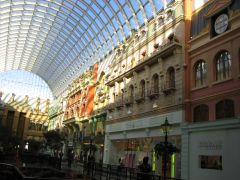
\includegraphics[width=.45\linewidth]{gfx/example_1}} \quad
        \subfloat[Pan ma signo.]
        {\label{fig:example-b}%
         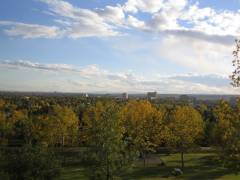
\includegraphics[width=.45\linewidth]{gfx/example_2}} \\
        \subfloat[Methodicamente o uno.]
        {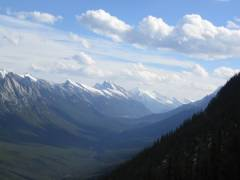
\includegraphics[width=.45\linewidth]{gfx/example_3}} \quad
        \subfloat[Titulo debitas.]
        {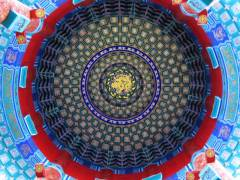
\includegraphics[width=.45\linewidth]{gfx/example_4}}
        \caption[Tu duo titulo debitas latente]{Tu duo titulo debitas
        latente.}\label{fig:example}
\end{figure}


%*****************************************
%*****************************************
%*****************************************
%*****************************************
%*****************************************

%************************************************
\chapter{Current mobile Platforms}\label{ch:m_plats} % $\mathbb{ZNR}$
%************************************************
\section{Android}
\spacedlowsmallcaps{Android} is a Linux based operating system specially designed for touchscreen devices like smartphones or tablets. It began as the brain-child of a new company called Android, Inc. back in 2003.

\begin{quotation}
Android, Inc. was founded in Palo Alto, California in October 2003 by Andy Rubin (co-founder of Danger), Rich Miner (co-founder of Wildfire Communications, Inc.), Nick Sears (once VP at T-Mobile), and Chris White (headed design and interface development at WebTV) to develop, in Rubin's words "smarter mobile devices that are more aware of its owner's location and preferences". The early intentions of the company were to develop an advanced operating system for digital cameras, when it was realised that the market for the devices was not large enough, and diverted their efforts to producing a smartphone operating system to rival those of Symbian and Windows Mobile (Apple's iPhone had not been released at the time). Despite the past accomplishments of the founders and early employees, Android Inc. operated secretly, revealing only that it was working on software for mobile phones. That same year, Rubin ran out of money. Steve Perlman, a close friend of Rubin, brought him \$10,000 in cash in an envelope and refused a stake in the company.
\cite{wikipedia:android}
\end{quotation}

Google bought Android, Inc. in 2005 and made it a wholly owned subsidiary. The most important employees stayed and started working on what later would become the Android Operating System.

Up until the release of the first Android Device on October \nth{22}, 2008, Google conducted secret meetings with many handset and chip manufacturers to discuss the creation of a new consortium, the Open Handset Alliance, with the goal to develop open standards for mobile devices. The Alliance was unveiled on November \nth{5}, 2007.\footnote{\url{http://www.openhandsetalliance.com/press_110507.html}}


After the first device with Android, the HTC Dream, was released there has been a major surge of devices using Android. Hardware manufacturers from all over the world have chosen Android as their favourite operating system, not only for smartphones and tablets but also for embedded devices like the Cotton Candy Stick from FXI Technologies and even gaming consoles like the Ouya. %They have gone the Android route to give their devices a robust and secure operating system.


The development of system features and other components has been done at a steady pace, releasing new versions of the OS every couple of months. The team has chosen to give colourful names to each release, always in alphabetical order and always named after a dessert or a sweet treat. A closer look at \autoref{fig:android1} and \autoref{fig:android2} should give you  better overview over the different versions of Android and what each new version brought forth.   

\begin{figure}
    \hbox{
        \hspace{-4em}
        {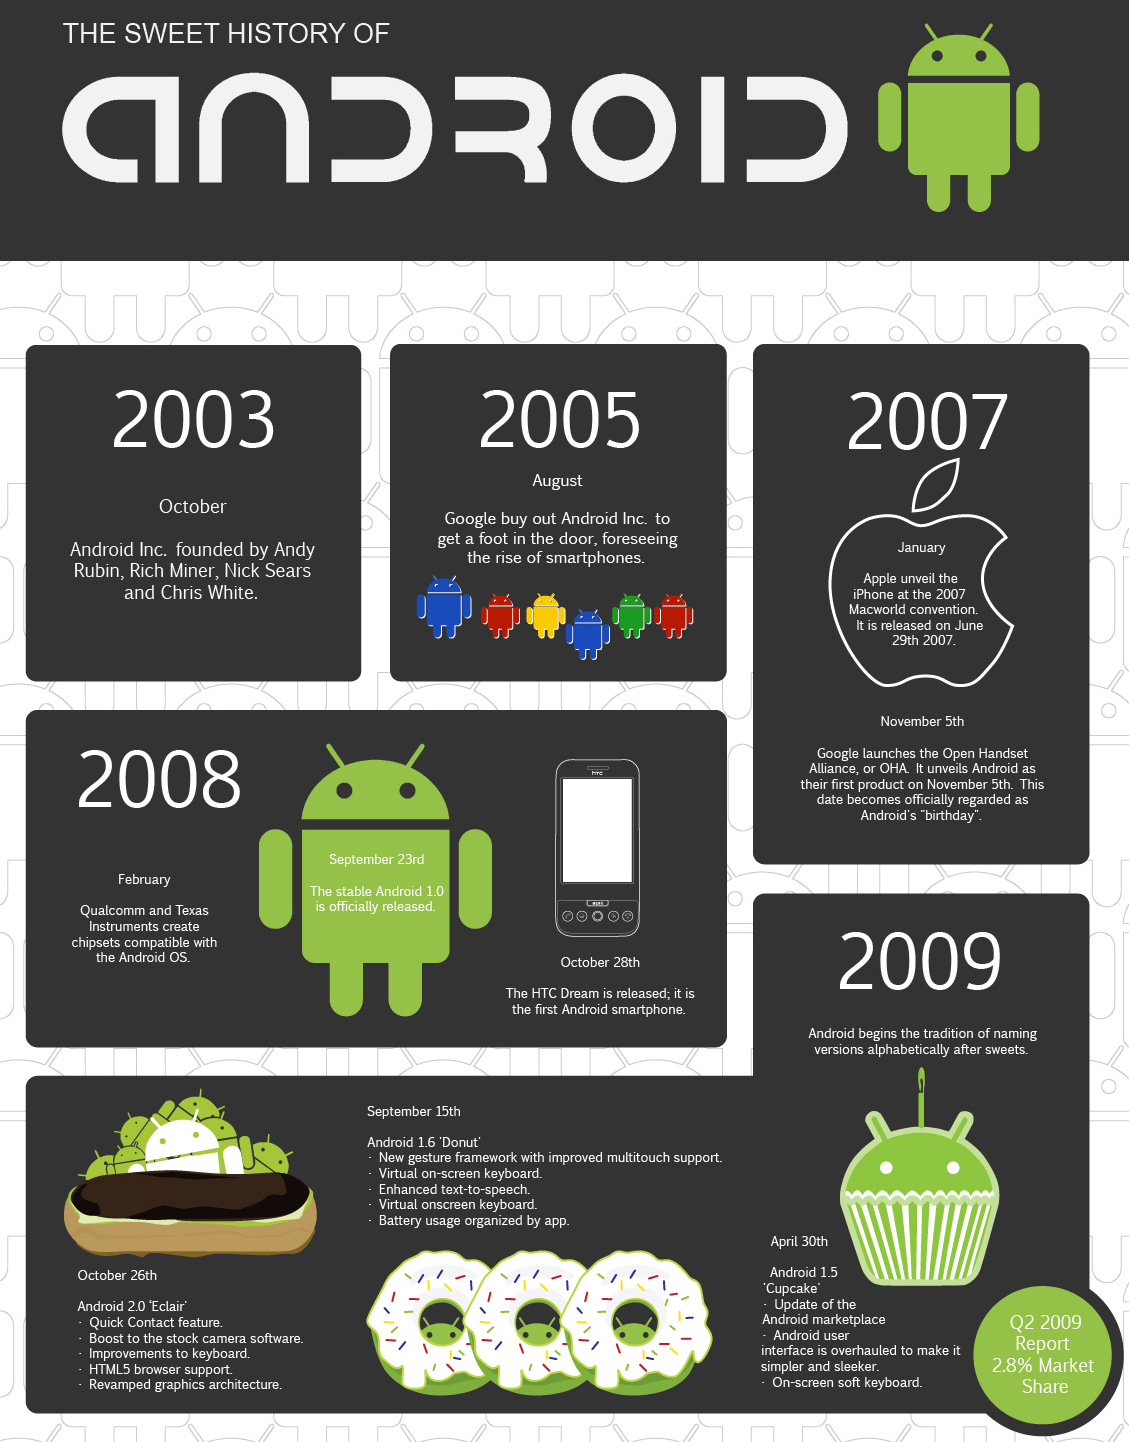
\includegraphics[width=1.5\linewidth]{gfx/android-history1}}
        \caption[Visual History of Android, Part 1]{Visual History of Android}\label{fig:android1}
    }
\end{figure}
\begin{figure}
    \hbox{
        \hspace{-12em}
        {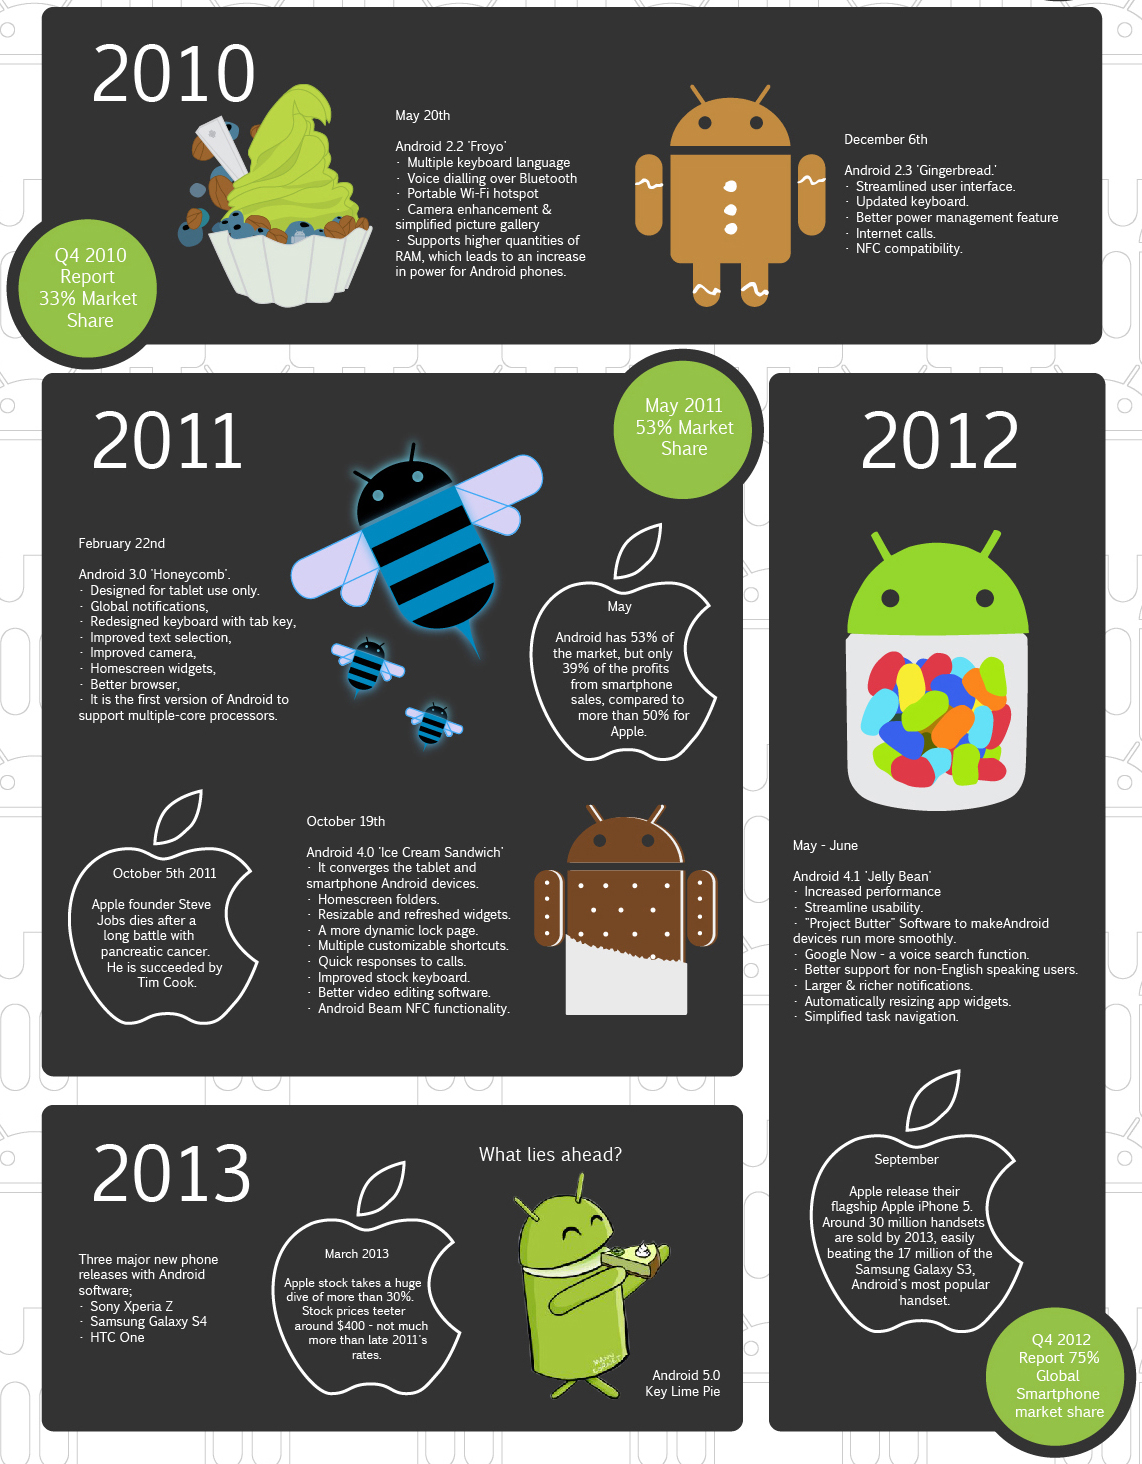
\includegraphics[width=1.55\linewidth]{gfx/android-history2}}
        \caption[Visual History of Android, Part 2]{Visual History of Android\footnotemark}\label{fig:android2}
    }
\end{figure}
\footnotetext{Source: \url{http://visual.ly/sweet-history-android}}\\

\subsection{The Android Open Source Project}
One of the best features and assets of Android is that it is 100\% Open Source. This allows everyone with the necessary knowledge to contribute to the development of the platform and also to modify it in every way you want.


This is exactly what the guys behind CyanogenMod have done. They took the regular Android Operating System and added many features and improvements to the core experience, making it the most popular unofficial Android OS.


But these types of modifications are not only common inside hobbyist communities, big corporations also contribute code to the Android Project. Some even modify the code so much, that it becomes almost unrecognisable. That is exactly what Amazon did. They took the Android OS and heavily modified it in order to install it in their Kindle Fire family of tablets.


Using an Open Source Model also guarantees Android an independent future from Google. Even if Google stops supporting \marginpar{Note: Google is unlikely to stop supporting Android} Android, the community will pick up the pieces and continue with its development and will guarantee its longevity.
 
\section{BlackBerry}
\section{iOS}
\begin{figure}[H]
    \begin{center}
        {\includegraphics[width=.90\linewidth]{gfx/ios-history}}
        \caption[Visual History of iOS]{Visual History of iOS\footnotemark}\label{fig:ios}
    \end{center}
\end{figure}
\footnotetext{Source: \url{http://visual.ly/history-ios}}\\

\section{Windows Phone}
\section{Other platforms worth noting}
The platforms mentioned above are the most popular ones. Together they control around 95\% of the mobile market, however, there are companies like Mozilla and Cononical that want to enter the competition and bring forth completely new ideas on what a mobile operating system should be.

\subsection{Firefox OS}
\spacedlowsmallcaps{Firefox OS} is Mozilla's entry to the mobile market. It hopes to revolutionise the mobile ecosystem by proposing that all applications for the device be programmed using Web Technologies.

\begin{quotation}
On July 25, 2011, Dr. Andreas Gal, Director of Research at Mozilla Corporation, announced the "Boot to Gecko" Project (B2G) on the mozilla.dev.platform mailing list. The project proposal was to "pursue the goal of building a complete, standalone operating system for the open web" in order to "find the gaps that keep web developers from being able to build apps that are – in every way – the equals of native apps built for the iPhone [iOS], Android, and WP7 [Windows Phone 7]." The announcement identified these work areas: new web APIs to expose device and OS capabilities such as telephone and camera, a privilege model to safely expose these to web pages, applications to prove these capabilities, and low-level code to boot on an Android-compatible device.
This led to much blog coverage. According to Ars Technica, "Mozilla says that B2G is motivated by a desire to demonstrate that the standards-based open Web has the potential to be a competitive alternative to the existing single-vendor application development stacks offered by the dominant mobile operating systems."
\cite{wikipedia:firefox}
\end{quotation}

In 2012 B2G was rebranded as Firefox OS in honour of the company's flagship product, the Firefox Web Browser.


Some preview units have been shipped to journalists and developers, in order to gain some traction, but the system has not come to production, yet. 

\begin{quotation}
In February 2013, Mozilla announced plans for global commercial roll-out of Firefox OS. Mozilla announced at a press conference before the start of Mobile World Congress in Barcelona that the first wave of Firefox OS devices will be available to consumers in Brazil, Colombia, Hungary, Mexico, Montenegro, Poland, Serbia, Spain and Venezuela. Firefox have also announced that LG Electronics, ZTE, Huawei and TCL Corporation have committed to making Firefox OS devices.
\cite{wikipedia:firefox}
\end{quotation}

 

\subsection{Ubuntu Phone}
\spacedlowsmallcaps{Ubuntu Phone} is Conical's horse in the mobile race. With it, Canonical hopes to disturb the mobile market by offering a single operating system capable of being a Mobile OS and a Desktop OS. As Canonical's own website puts it, 

\begin{quotation}
High-end smartphones have a brain as powerful as ultra-light laptops. Ubuntu uniquely enables a new category of convergence device – phones that dock to become full PCs and thin clients; enabling enterprise IT departments to replace phones, thin clients and laptops with a single secure corporate device.\\

Operators targeting the enterprise market with LTE can now deliver a full laptop/phone solution, with Windows apps delivered over LTE from the corporate data center. And operators in emerging markets can deliver desktop applications to the converged device over LTE as a premium data service.\footnote{\url{http://www.ubuntu.com/phone/operators-and-oems}}
\end{quotation}


\spacedlowsmallcaps{Ubuntu Phone} is still in the early stages of development, but has already gained the backing of major OEM's and carriers around the world. Once it hits the market, it will become the next player to watch, doubtlessly bringing new ideas and features to the table.  
















 
%************************************************
\chapter{History of MHM Systemhaus GmbH}\label{ch:mhm_history}
%************************************************
\cleardoublepage
\ctparttext{Part 2 Text}
\part{Developing multi-platform applications}
%************************************************
\chapter{Frameworks for multi-platform development}\label{ch:frameworks}
%************************************************
There are numerous frameworks that have been developed over the years to facilitate the creation of multi-platform applications. Just like in the 90s when vendors saw market opportunities in releasing multi-platform applications for the desktop, most of the solutions available for cross-platform mobile development are of the commercial nature.


However, \marginpar{PhoneGap is the commercial name of the Apache Cordova Open Source Project.} some open source players do exist. They have been gaining popularity and better features over time, some even have been backed by bigger organisations offering both free and commercial packages. Examples worth noting in this category are PhoneGap, backed by Adobe and MonoTouch, backed by Xamarin.
\graffito{Mono is an open source implementation of Microsoft's .NET Framework.}

\section{Types of Frameworks}
When it comes to choosing the adequate framework to use for the development of your application there are many options that vary in features, pricing and support; but they can all be sorted into three different categories, based on the type of application they produce at the end. These categories are:
\begin{enumerate}
    \item HTML5 Web Applications (\autoref{sec:web_app})
    \item Hybrid Applications (\autoref{sec:hyb_app})
    \item Pseudo-Native Applications (\autoref{sec:pseudo_app})
\end{enumerate}

You should always keep in mind the advantages and drawbacks of each when choosing which type of framework is the best for you needs, but let us take a look at \autoref{tab:frameworks} first. It should give you an overview over the technologies used and the type of applications produced by the most popular cross-platform frameworks. We will discuss each type in detail later on.\newline
\begin{table}[H]
    \myfloatalign
  \begin{tabularx}{\textwidth}{Xll} \toprule
    \tableheadline{Name} & \tableheadline{Language} & \tableheadline{Type}\\ 
    \midrule
    Any web framework & HTML5 \& Javascript & Web App\\
    Corona SDK & Lua & Pseudo-Native\\
    Icenium & Javascript & Hybrid\\
    Intel XDK & Javascript & Hybrid\\
    PhoneGap & Javascript & Hybrid\\
    Rhodes & Ruby \& Javascript & Hybrid\\
    Titanium SDK & Javascript & Hybrid\\
    Xamarin & C\# + Native UI & Pseudo-Native\\      
    %\midrule
    \bottomrule
  \end{tabularx}
  \caption[Characteristics of the most popular cross-platform frameworks]{Overview of some characteristics of the most popular cross-platform frameworks}  \label{tab:frameworks}
\end{table}  

As \autoref{tab:frameworks} lets us see, the majority of available frameworks seem to be those that deliver a hybrid application. This phenomenon can be explained by what \citeauthor{allen:2010} express in their book about Cross-Platform Development:
\begin{quotation}
The innovation in cross-platform frameworks for smartphone applications surpasses the patterns of abstraction seen in the cross-platform desktop frameworks of the 1990s. These new smartphone frameworks are influenced by the rapid application development techniques we are seeing in web development today. There are three specific techniques in web application development that are borrowed for these non-web frameworks: 1) layout with mark-up (HTML/CSS); 2) using URLs to identify screen layouts and visual state; and 3) incorporating dynamic languages, such as Javascript and Ruby.\\

A generation of designers and user interface developers are fluent in HTML and CSS for layout and construction of visual elements. Additionally, addressing each screen by a unique name in a sensible hierarchy (URL) with a systemized way of defining connections between them (links and form posts) has created a lingua franca understood by visual and interactions designers, information architects, and programmers alike. This common language and its standard implementation patterns led to the development of frameworks and libraries that significantly speed application development on the Web. These patterns are now being applied to the development of mobile applications as common techniques by individual developers as well as in cross-platform frameworks.
\cite[p. 23]{allen:2010}
\end{quotation}
Before we dive into each type of framework, \autoref{fig:hybrid_native} should give you a better overview over the capabilities of each of them.\\

\marginpar{\autoref{fig:hybrid_native}: The 'Native' label also applies to Pseudo-Native}
\begin{figure}[H]
    \begin{center}
        {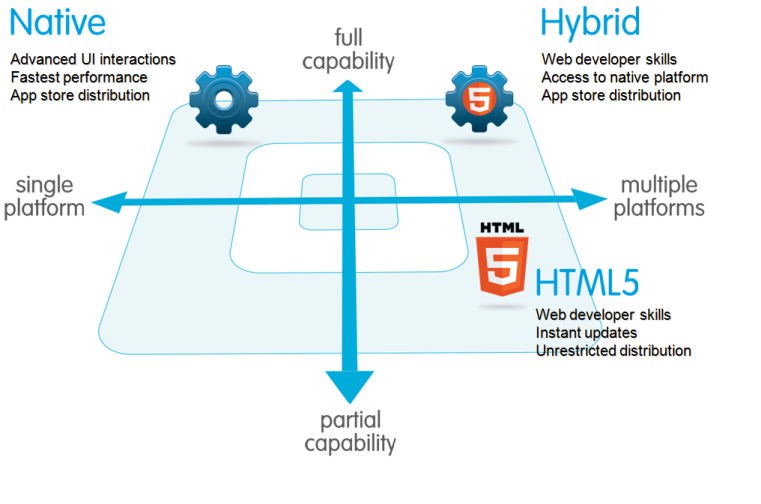
\includegraphics[width=1\linewidth]{gfx/Native_html5_hybrid}}
        \caption[Overview of app capabilities. Native vs. Hybrid vs. HTML5]{Overview of app capabilities. Native vs. Hybrid vs. HTML5\footnotemark}\label{fig:hybrid_native}
    \end{center}
\end{figure}
\footnotetext{Source: \url{http://wiki.developerforce.com/page/Native,_HTML5,_or_Hybrid:_Understanding_Your_Mobile_Application_Development_Options}}\\

\subsection{HTML5 Web Applications}\label{sec:web_app}
Just as any other website, \spacedlowsmallcaps{HTML5 Web Applications} can be developed in any language that can be translated to HTML code on runtime. Some examples of these languages are \emph{Ruby, PHP, Python, JSP} or just plain HTML. Some of the most popular web development frameworks, like Ruby on Rails or Synfony\marginpar{Synfony is an MVC Framework for PHP, similar, but not quite as powerful as Rails.}, are very well suited for the development of Web Applications for Mobile Devices.


But having HTML code is not everything, you still need to make it look good in the smaller screen of cellphones and tablets. That's where CSS3 comes to the rescue. With CSS3 you define the look and feel of the application, but you need to define specific rules for devices with a smaller resolution. This can be accomplished in two ways:
\begin{enumerate}
    \item Responsive CSS3 Design
    \item Separate Domain and CSS files for mobile devices
\end{enumerate}
\spacedlowsmallcaps{Responsive CSS3 Design} means you need to distinguish between the different screen sizes and define different rules and properties for each inside your CSS files. With responsive design, changes in screen orientation can also be translated to a different layout, e.g. changing the width of tables or the arrangement of images.


With \spacedlowsmallcaps{Separate Files} you will have to redirect visitors using a mobile device to a different domain and have that domain serve the corresponding CSS files. This approach has some caveats, the most obvious one being the overhead of a different domain and the fact that if you want your layout to react to screen dimension changes, you will most likely need to implement some sort of responsive design.   
 

These frameworks, however, cannot run inside the mobile device; they need to run in a server, which means that the only way to access the application is through a web browser.


This line of action is best suited for smaller projects that want to present their website or web application in a better way to mobile users, but don't have the resources to hire a full time application developer. They can use the designer they have at hand and just optimise their online presence for portable devices.

\subsection{Hybrid Applications}\label{sec:hyb_app}
\begin{quotation}
Before any cross-platform frameworks existed, many developers found that embedding Web UI in a native application was a practical way to develop mobile applications quickly and make cross-platform applications easier to maintain. The user interface for mobile applications tends to be presented as a series of screens. From a high level, the mobile UI can be thought of as having the same flow-of-control as a traditional web site or web application. \cite[p. 28]{allen:2010}
\end{quotation}

\spacedlowsmallcaps{Hybrid Applications} are, in a lot aspects, very similar to HTML5 Web Applications. Both rely on HTML, Javascript and CSS for the definition of the UI, but the edge of Hybrid Applications lies in the way they are packaged.


With \spacedlowsmallcaps{Hybrid Applications} the HTML, et al. are contained within a native application, that allows the framework's API to communicate with the operating system, thus leveraging most of the native features the hardware has to offer, e.g. access to the camera, the accelerometer, the GPS, local storage, security features, etc. Access to these features is accomplished via a wrapper that is programmed in each platform's native language and exposes specific methods to an API that is accessible from the HTML side.


By having access to these features, Hybrid Applications can behave like native applications and, since they are contained within a native package, there is no need for the user to open a web browser. The user never needs to know whether the application is native or hybrid, everything is just one seamless experience. It also gives you the advantage of distributing your application via the platform's store.


This approach gives you many added benefits over a normal HTML5 Application, with little trade-off. There is a learning curve when dealing with the programming frameworks, but the design and layout are still done in HTML and CSS. One of the main benefits you get is that you now have the possibility to make your application available offline and of course the access to system features like push notifications and background services. It is best suited for projects that want to offer more functionality with their mobile applications and are willing to invest some time in learning the new framework.  

\subsection{Pseudo-Native Applications}\label{sec:pseudo_app}
\spacedlowsmallcaps{Pseudo-Native Applications} are completely different from the other two types. They do not rely on HTML for the UI or on Javascript for communication with native features. These applications are compiled to native code and appear to the device as full native applications. 
















  
%************************************************
\chapter{Introduction}\label{ch:introduction}
%************************************************
%************************************************
\chapter{Placeholder}\label{ch:introduction}
%************************************************
%\addtocontents{toc}{\protect\clearpage} % <--- just debug stuff, ignore

\ctparttext{Part 3 Text}
\part{Mobile environments \& the Cloud}
%************************************************
\chapter{Placeholder}\label{ch:introduction}
%************************************************
%************************************************
\chapter{Placeholder}\label{ch:introduction}
%************************************************
%************************************************
\chapter{Placeholder}\label{ch:introduction}
%************************************************
%************************************************
\chapter{Placeholder}\label{ch:introduction}
%************************************************
%************************************************
\chapter{Placeholder}\label{ch:introduction}
%************************************************

\ctparttext{A real world approach}
\part{A real world approach}
%************************************************
\chapter{Placeholder}\label{ch:introduction}
%************************************************
%************************************************
\chapter{Placeholder}\label{ch:introduction}
%************************************************
%************************************************
\chapter{Influence of the Cloud in Mobile Applications}\label{ch:influence}
%************************************************

The Cloud has had a big impact and influence on how mobile applications have evolved and changed over the past few years. Before the introduction of the Cloud we know today, mobile applications were fairly simple and often focused in productivity and personal organization. The first \ac{PDA} devices did just that. They came with a set of applications developed by the manufacturer and the user could not change the installed applications or add new ones. With the dawn of the mobile internet a new wave 
%************************************************
\chapter{Placeholder}\label{ch:introduction}
%************************************************
%\include{multiToC} % <--- just debug stuff, ignore for your documents
% ********************************************************************
% Backmatter
%*******************************************************
\appendix
\cleardoublepage
%\part{Appendix}
%********************************************************************
% Appendix
%*******************************************************
% If problems with the headers: get headings in appendix etc. right
%\markboth{\spacedlowsmallcaps{Appendix}}{\spacedlowsmallcaps{Appendix}}
\chapter{Appendix Test}
Lorem ipsum at nusquam appellantur his, ut eos erant homero
concludaturque. Albucius appellantur deterruisset id eam, vivendum
partiendo dissentiet ei ius. Vis melius facilisis ea, sea id convenire
referrentur, takimata adolescens ex duo. Ei harum argumentum per. Eam
vidit exerci appetere ad, ut vel zzril intellegam interpretaris.

Errem omnium ea per, pro congue populo ornatus cu, ex qui dicant
nemore melius. No pri diam iriure euismod. Graecis eleifend
appellantur quo id. Id corpora inimicus nam, facer nonummy ne pro,
kasd repudiandae ei mei. Mea menandri mediocrem dissentiet cu, ex
nominati imperdiet nec, sea odio duis vocent ei. Tempor everti
appareat cu ius, ridens audiam an qui, aliquid admodum conceptam ne
qui. Vis ea melius nostrum, mel alienum euripidis eu.

\section{Appendix Section Test}
Ei choro aeterno antiopam mea, labitur bonorum pri no. His no decore
nemore graecis. In eos meis nominavi, liber soluta vim cu. Sea commune
suavitate interpretaris eu, vix eu libris efficiantur.

\graffito{More dummy text.}
Nulla fastidii ea ius, exerci suscipit instructior te nam, in ullum
postulant quo. Congue quaestio philosophia his at, sea odio autem
vulputate ex. Cu usu mucius iisque voluptua. Sit maiorum propriae at,
ea cum primis intellegat. Hinc cotidieque reprehendunt eu nec. Autem
timeam deleniti usu id, in nec nibh altera.

\section{Another Appendix Section Test}
Equidem detraxit cu nam, vix eu delenit periculis. Eos ut vero
constituto, no vidit propriae complectitur sea. Diceret nonummy in
has, no qui eligendi recteque consetetur. Mel eu dictas suscipiantur,
et sed placerat oporteat. At ipsum electram mei, ad aeque atomorum
mea.

\begin{table}
    \myfloatalign
  \begin{tabularx}{\textwidth}{Xll} \toprule
    \tableheadline{labitur bonorum pri no} & \tableheadline{que vista}
    & \tableheadline{human} \\ \midrule
    fastidii ea ius & germano &  demonstratea \\
    suscipit instructior & titulo & personas \\
    %postulant quo & westeuropee & sanctificatec \\
    \midrule
    quaestio philosophia & facto & demonstrated \\
    %autem vulputate ex & parola & romanic \\
    %usu mucius iisque & studio & sanctificatef \\
    \bottomrule
  \end{tabularx}
  \caption[Autem usu id]{Autem usu id.}
  \label{tab:moreexample}
\end{table}

Ei solet nemore consectetuer nam. Ad eam porro impetus, te choro omnes
evertitur mel. Molestie conclusionemque vel at, no qui omittam
expetenda efficiendi. Eu quo nobis offendit, verterem scriptorem ne
vix.

  
\begin{lstlisting}[float,caption=A floating example]
for i:=maxint to 0 do
begin
{ do nothing }
end;
\end{lstlisting}
%********************************************************************
% Other Stuff in the Back
%*******************************************************
\cleardoublepage%********************************************************************
% Bibliography
%*******************************************************
% work-around to have small caps also here in the headline
\manualmark
\markboth{\spacedlowsmallcaps{\bibname}}{\spacedlowsmallcaps{\bibname}} % work-around to have small caps also
%\phantomsection 
\refstepcounter{dummy}
\addtocontents{toc}{\protect\vspace{\beforebibskip}} % to have the bib a bit from the rest in the toc
\addcontentsline{toc}{chapter}{\tocEntry{\bibname}}
\bibliographystyle{plainnat}
\label{app:bibliography} 
\bibliography{Bibliography}
\cleardoublepage\pagestyle{empty}

\hfill

\vfill


\pdfbookmark[0]{Colophon}{colophon}
\section*{Colophon}
This document was typeset using the typographical look-and-feel \texttt{classicthesis} developed by Andr\'e Miede. 
The style was inspired by Robert Bringhurst's seminal book on typography ``\emph{The Elements of Typographic Style}''. 
\texttt{classicthesis} is available for both \LaTeX\ and \mLyX: 
\begin{center}
\url{http://code.google.com/p/classicthesis/}
\end{center}
Happy users of \texttt{classicthesis} usually send a real postcard to the author, a collection of postcards received so far is featured here: 
\begin{center}
\url{http://postcards.miede.de/}
\end{center}
 
\bigskip

\noindent\finalVersionString

%Hermann Zapf's \emph{Palatino} and \emph{Euler} type faces (Type~1 PostScript fonts \emph{URW
%Palladio L} and \emph{FPL}) are used. The ``typewriter'' text is typeset in \emph{Bera Mono}, 
%originally developed by Bitstream, Inc. as ``Bitstream Vera''. (Type~1 PostScript fonts were made 
%available by Malte Rosenau and
%Ulrich Dirr.)

%\paragraph{note:} The custom size of the textblock was calculated
%using the directions given by Mr. Bringhurst (pages 26--29 and
%175/176). 10~pt Palatino needs  133.21~pt for the string
%``abcdefghijklmnopqrstuvwxyz''. This yields a good line length between
%24--26~pc (288--312~pt). Using a ``\emph{double square textblock}''
%with a 1:2 ratio this results in a textblock of 312:624~pt (which
%includes the headline in this design). A good alternative would be the
%``\emph{golden section textblock}'' with a ratio of 1:1.62, here
%312:505.44~pt. For comparison, \texttt{DIV9} of the \texttt{typearea}
%package results in a line length of 389~pt (32.4~pc), which is by far
%too long. However, this information will only be of interest for
%hardcore pseudo-typographers like me.%
%
%To make your own calculations, use the following commands and look up
%the corresponding lengths in the book:
%\begin{verbatim}
%    \settowidth{\abcd}{abcdefghijklmnopqrstuvwxyz}
%    \the\abcd\ % prints the value of the length
%\end{verbatim}
%Please see the file \texttt{classicthesis.sty} for some precalculated 
%values for Palatino and Minion.
%
%    \settowidth{\abcd}{abcdefghijklmnopqrstuvwxyz}
%    \the\abcd\ % prints the value of the length





% ********************************************************************
% Game Over: Restore, Restart, or Quit?
%*******************************************************
\end{document}
% ********************************************************************
